\chapter{The X-HEEP Platform}

    \section{Introduction}
    \label{sec:introduction}

        % Pre-introduction: The other sections are moved to the introduction chapter
        As design space exploration for TinyAI systems progresses from early functional validation to realistic deployment scenarios, prototyping infrastructures must evolve to meet stricter fidelity and implementation requirements. The FEMU framework~\cite{femu} addresses this need by enabling early-stage evaluation of systems through a combination of virtualized software components and reconfigurable hardware. A central element within FEMU is the host, part of the heterogeneous system under development, which orchestrates control and communication tasks, as well as interfaces with custom accelerators~\cite{e-gpu, asip, oe-cgra, blade}. To be effective, this host must be synthesizable, configurable, and capable of adapting to the diverse architectural needs imposed by a wide range of accelerators.

        % Problem: Accelerator Requirements
        Each domain-specific accelerator exhibits distinct design requirements, which stem from the highly variable computational, memory, and energy constraints imposed by its respective applications. These requirements often span a wide range of metrics, including memory size, logic area, operating frequency, peak throughput, and power consumption~\cite{x-heep}. For instance, accelerators designed for neural networks~\cite{cnn-accel} may demand high parallelism and substantial memory bandwidth, whereas cryptographic units~\cite{keccak} might prioritize low-latency execution and secure data handling. Similarly, accelerators targeting biomedical signal processing~\cite{oe-cgra, blade} may require fine-grained power control to sustain energy autonomy across long acquisition windows.

        % Problem: Configurable and Extendible Host Platforms
        To support this diversity in a scalable and maintainable manner, the host platform must itself be adaptable. Rigid or monolithic system architectures severely limit the ability to integrate such heterogeneous accelerators efficiently, often leading to suboptimal trade-offs in performance and energy. Instead, a highly configurable host design is necessary, one that allows designers to explore and tune architectural parameters across multiple dimensions. These include, but are not limited to, selecting different central processing units (CPUs) to balance performance and power efficiency; choosing bus topologies and memory hierarchies that match the expected communication patterns and data reuse behaviors of accelerators; scaling internal memory sizes and banking strategies to meet the working set requirements; and exposing appropriate peripheral interfaces to support diverse sensing, actuation, or off-chip memory use cases.

        Furthermore, to maximize energy efficiency, particularly in TinyAI scenarios, fine-grained power management strategies must be supported at the architectural level. This involves the delineation of multiple power and clock domains, the ability to selectively power-gate or clock-gate idle components, and mechanisms to enable retention of critical state when subsystems are in low-power modes. Ultimately, a truly effective host platform must serve not just as a controller or coordinator, but as a configurable infrastructure that can adapt to the highly specific hardware and software demands of the integrated accelerators and the target applications they support.

        % SOTA: Host Platforms - Limitation: Configurability
        Despite the growing availability of open-source host platforms, many of these efforts primarily focus on the CPU core, offering limited infrastructure beyond the processor itself. While valuable for early experimentation, such CPU-centric designs fall short of addressing the broader architectural needs required for seamless accelerator integration in resource-constrained systems. In particular, state-of-the-art hosts~\cite{pulpissimo, opentitan, blackparrot} often lack the configurability necessary to adapt internal components, such as memory hierarchy, interconnect topology, and peripheral interfaces, to the requirements imposed by heterogeneous accelerators~\cite{e-gpu, asip, oe-cgra, blade}. This lack of flexibility constrains the exploration of system-level trade-offs and limits the ability to design application-specific solutions optimized for performance, area, or energy consumption.

        % SOTA: Host Platforms - Limitation: Extendability
        Moreover, the integration of external accelerators is frequently impeded by inadequate support for extensible interfaces~\cite{blackparrot, chipyard, opentitan}, limited communication bandwidth, or the absence of hardware hooks for interrupt handling and low-power control. These architectural omissions force hardware developers to perform extensive manual modifications at the register-transfer level (RTL) to retrofit support for new accelerators, significantly increasing design complexity and verification overhead. Often, this process involves forking the original platform repository, introducing architectural changes to match application requirements, and maintaining a parallel development branch. Over time, this results in high maintenance costs, reduced interoperability, and the fragmentation of the open-source ecosystem.

        % Approach
        To mitigate these challenges and promote sustainable development practices, it is essential to systematically address the configurability and extendability of host platforms. Platforms must evolve beyond fixed-function implementations and adopt modular and reusable design principles that accommodate a diverse range of accelerators and workloads. By lowering the architectural barrier to integration and reducing the cost of platform customization, such designs can accelerate the adoption of open-source hardware in edge computing domains and foster innovation in TinyAI heterogeneous systems.

        % My Solution: The X-HEEP Platform
        To address the limitations outlined above, this chapter introduces the eXtendible Heterogeneous Energy Efficient Platform (\mbox{X-HEEP})~\cite{x-heep, x-heep_1, x-heep_2}, an open-source, highly configurable, and extendible platform designed to facilitate the integration and exploration of TinyAI accelerators. \mbox{X-HEEP} is built as a modular RISC-V-based host that provides a scalable environment for realizing robust heterogeneous systems. It leverages silicon-validated IP blocks from leading open-source initiatives, including the PULP platform, the OpenHW Group, and the OpenTitan project. These foundations ensure compatibility with widely adopted tools and software stacks while enabling the reuse of thoroughly verified IPs and software extensions, thereby accelerating development and reducing validation costs.
        
        % Feature: Configurability
        To support application-specific tuning, \mbox{X-HEEP} offers a comprehensive set of internal configuration options. Designers can select among various RISC-V CPU types depending on workload requirements~\cite{zeroriscy}, choose suitable bus topologies and addressing modes to meet bandwidth and locality constraints, adjust the size and organization of internal memory to match data storage needs, and instantiate only the peripherals required by the target application. This high degree of customization allows the platform to satisfy diverse constraints in area, latency, and energy consumption across a wide spectrum of TinyAI use cases.
        
        % Feature: XAIF Interface
        A central enabler of this flexibility is the eXtendible Accelerator InterFace (XAIF), a modular integration layer that provides standardized connectivity for a broad range of accelerators, each with potentially unique area, power, performance, and memory interface requirements. XAIF consolidates key architectural elements, such as bus connectivity, interrupt signaling, and low-power coordination, into a unified interface abstraction.
        
        % Feature: Power-reduction Strategies
        Given the strict energy efficiency requirements of TinyAI systems, \mbox{X-HEEP} incorporates low-power techniques at the architectural level. These include clock-gating, power-gating, and memory retention strategies, all tightly integrated with the XAIF interface. As a result, both the host and its connected accelerators can be dynamically managed to minimize switching and leakage power, achieving energy proportionality across the system. This power management strategy makes \mbox{X-HEEP} particularly suitable for deployment in long-running, battery-operated applications where energy autonomy is essential.
        
        % Feature: Support for FPGA and ASIC
        In addition to architectural extensibility, \mbox{X-HEEP} is designed to support rapid design space exploration across multiple implementation backends. Configurations can be instantiated and evaluated on field-programmable gate array (FPGA) targets for early-stage prototyping, on RTL simulators for cycle-accurate functional validation, or within mixed-level SystemC simulations for high-level performance modeling. This multi-level flow provides essential feedback throughout the hardware–software co-design process and enables incremental development toward silicon-ready implementations.
        
        To validate the architectural principles and configurability features of the proposed \mbox{X-HEEP} platform, and to demonstrate its applicability to real-world edge scenarios, a representative integration example targeting bio-signal processing is presented. This domain is highly relevant for TinyAI, as it often involves prolonged acquisition periods in which physiological signals are sampled at low rates from external biosensors and stored in memory, followed by compute-intensive processing phases involving digital signal processing (DSP), machine learning (ML), or deep learning (DL) techniques.
        
        To support such heterogeneous workloads, two domain-specific accelerators are instantiated: a coarse-grained reconfigurable array (CGRA)~\cite{oe-cgra} and an in-memory computing (IMC) accelerator~\cite{blade}, both previously shown to reduce energy consumption in healthcare tasks~\cite{bio_apps, co-design_vision}. These accelerators are seamlessly integrated into the \mbox{X-HEEP} host through the XAIF interface, demonstrating the ability of the platform to accommodate diverse accelerator requirements. The system is configured with the CV32E20 RISC-V core~\cite{zeroriscy}, eight banks of \SI{32}{\kibi\byte} SRAM in contiguous addressing mode, and eleven independent power domains, including those of the external accelerators, each supporting fine-grained clock- and power-gating.
        
        The complete system, named \textsc{HEEPocrates}~\cite{heepocrates}, is implemented across multiple Xilinx FPGA platforms, such as Zynq-7020, Zynq UltraScale+, and Artix-7, for rapid prototyping and system exploration. For final validation and energy profiling, the design is fabricated in TSMC \SI{65}{\nano\meter} CMOS technology, demonstrating that \mbox{X-HEEP} supports not only high configurability and accelerator extensibility but also real-world deployment in silicon, with competitive figures in area, power, and performance.

        The key contributions of this chapter are summarized as follows:

        \vspace{-1em}
        \begin{itemize}
            \item \mbox{X-HEEP}~\cite{x-heep}: A configurable and extensible RISC-V host platform for supporting the exploration of TinyAI accelerators.
    
            \item \mbox{XAIF}: A highly adaptable accelerator interface that enables straightforward and flexible integration of accelerators with varying interface constraints.

            \item Extensive internal configurability that enables fine-grained optimizations to match application requirements.
    
            \item \mbox{HEEPocrates}~\cite{heepocrates}: A full system-on-chip (SoC) implementation in TSMC \SI{65}{\nano\meter} low-power CMOS technology, featuring the integration of a CGRA~\cite{oe-cgra} and an IMC~\cite{blade} accelerator as a real-world use case of \mbox{X-HEEP}.
    
            \item A publicly released open-source repository including the complete code and documentation of \mbox{X-HEEP} to support future research on TinyAI heterogeneous systems.\footnote{The complete code and documentation of the \mbox{X-HEEP platform} are available at \url{https://github.com/esl-epfl/x-heep}.}
        \end{itemize}
        \vspace{-1em}
        
        The remainder of this chapter is organized as follows. Section~\ref{sec:related_work} reviews relevant open-source accelerators and host platforms, highlighting their main characteristics and integration limitations. Section~\ref{sec:x-heep_platform} introduces the configurability and extendability features of the \mbox{X-HEEP} platform. Section~\ref{sec:heepocrates} illustrates a real-world integration example, \mbox{HEEPocrates}, targeting bio-signal processing workloads. Section~\ref{sec:x-heep_based_systems} analyzes the most relevant \mbox{X-HEEP}-based systems. Section~\ref{sec:experimental_setup} presents the experimental setup, while Section~\ref{sec:experimental_results} the experimental results. Finally, Section~\ref{sec:conclusions} summarizes our findings.

    \section{Related Work}
    \label{sec:related_work}
    
        This section presents a comprehensive survey of the current state-of-the-art in the design and integration of edge accelerators within host platforms. The review is organized into two main parts. The first part introduces a classification of open-source accelerators based on their interfacing and operational characteristics. This taxonomy serves as a foundation for understanding the architectural diversity and the design trade-offs associated with different accelerator types. The second part evaluates prominent open-source host platforms that act as integration targets for edge-computing accelerators. Each platform is assessed in terms of its configurability, extensibility, and suitability for heterogeneous system integration. The analysis highlights persistent limitations in existing solutions, particularly regarding flexibility and energy efficiency, thereby motivating the development of a new class of host platforms specifically tailored to the requirements of the TinyAI domain.
    
        \subsection{Interfacing Edge Accelerators}
    
            Edge accelerators exhibit a high degree of heterogeneity, as they target a broad range of application domains, including cryptography, signal processing, neural networks, and control systems. As a result, their integration requirements vary significantly in terms of bus connectivity, configurability, and communication bandwidth. The interfacing patterns of existing accelerators can be categorized into four primary classes: \emph{slave-only}, \emph{master/slave hybrid}, \emph{master-only}, and \emph{co-processors}. This classification formalizes the hardware–software boundary and supports the design of a unified interface for scalable and efficient accelerator integration.

            \vspace{-1em}
            \subsubsection*{Slave-Only Accelerators}
            
                Slave-only accelerators are defined by the presence of one or more slave ports, typically used for register-level access or memory-mapped control interfaces. These IP blocks rely on the host CPU or a direct memory access (DMA) engine to transfer data between main memory and the internal buffers of the accelerator before execution. Synchronization is commonly managed through interrupts or status registers.
                
                A representative example is the Keccak hashing accelerator~\cite{keccak}, which exposes two distinct \SI{32}{\bit} slave ports: one for accessing the register file that controls execution, and another for reading and writing private data memory. This separation enables modular interaction between control and data planes but shifts the responsibility of data movement entirely to the host.
                
                Another example is the C-SRAM accelerator~\cite{cea_imc}, an in-memory compute architecture that interprets write transactions as encoded instructions. A single \SI{32}{\bit} slave port serves as both a configuration and a command interface, with the address and data fields jointly encoding memory-embedded operations. This design prioritizes simplicity and energy efficiency but provides minimal autonomy, requiring extensive software orchestration.
                
                Although slave-only accelerators are typically compact and power-efficient, they require tight hardware-software coupling. As a result, the host platform must offer fine-grained control over address space mapping and interrupt management to support this integration model effectively.

            \vspace{-1em}
            \subsubsection*{Master/Slave Hybrid Accelerators}
            
                Hybrid accelerators represent a more autonomous class of IPs that integrate slave ports for configuration with master ports for direct access to shared memory. This architecture enables the accelerator to independently fetch input data and write back results, thereby reducing CPU intervention and improving overall throughput. Such designs are prevalent in high-performance domains, including DSP and domain-specific ML workloads.
                
                A representative example is the CGRA-based accelerator~\cite{oe-cgra}, which includes two \SI{32}{\bit} slave ports for configuration and instruction loading, along with four \SI{32}{\bit} master ports for parallel access to shared memory. With an aggregate bandwidth of \SI{128}{\bit}/cycle, this design illustrates the importance of multi-port interfacing for bandwidth-intensive applications.
                
                Another notable example is the PULP cluster~\cite{pulp_cluster}, a tightly coupled multi-core accelerator composed of four to eight CV32E40P RISC-V CPUs~\cite{ri5cy}. It features a slave port for control and data pre-loading, complemented by a shared \SI{64}{\bit} master port used for instruction fetching and DMA-driven data transfers. The cluster also includes shared scratchpad memory and an instruction cache, which combine high performance with software programmability.
                
                In the domain of application-specific designs, Echoes~\cite{fft} implements a fast Fourier transform (FFT) accelerator with eight \SI{32}{\bit} master ports, achieving a total bandwidth of \SI{256}{\bit}/cycle. Similarly, Marsellus~\cite{cnn} supports convolutional operations using nine master ports, delivering up to \SI{288}{\bit}/cycle. These architectures highlight the growing demands on memory bandwidth and underscore the need for sophisticated interconnect solutions on the host side.
                
                Reconfigurable fabrics such as embedded FPGAs (eFPGAs) also follow the hybrid model. For example, Arnold~\cite{arnold} features an eFPGA that can act as a control unit for off-chip IPs or perform local data pre-processing. It exposes a slave interface for runtime configuration and bitstream loading, enabling dynamic reconfiguration during execution.
                
                These hybrid accelerators require host platforms that support flexible slave interfaces, scalable master port integration, and robust infrastructure for clock domain crossing, synchronization, and advanced memory partitioning.
    
            \subsubsection*{Master-Only Accelerators}
            
                Master-only accelerators are fully autonomous and initiate all memory transactions exclusively through master ports. They do not rely on slave ports for configuration, as their behavior is typically defined by software stored in shared memory. This paradigm is well-suited to general-purpose compute engines that require minimal host involvement during execution.
                
                Typical examples include low-power RISC-V cores such as CV32E20, CV32E40X, and CV32E40P~\cite{zeroriscy}, as well as higher-performance processors like the Ariane core~\cite{ariane}. GPU-based designs such as Vortex~\cite{vortex} also adopt this model, functioning as self-managed compute engines capable of independently fetching both code and data from memory.
                
                Since these accelerators operate similarly to general-purpose processors, the host platform must provide instruction-level access to shared memory and ensure support for task scheduling and resource arbitration to enable safe and efficient execution.

            \subsubsection*{Tightly-Coupled Co-Processors}
            
                Tightly-coupled co-processors are designed as instruction set architecture (ISA) extensions to accelerate specific operations and are either integrated directly into the processor pipeline or connected via dedicated low-latency interfaces. This architecture enables the efficient offloading of micro-tasks from the main CPU with minimal communication overhead.
                
                Common application domains for such co-processors include floating-point arithmetic~\cite{fp}, posit number systems~\cite{posit}, post-quantum cryptography~\cite{pqcry}, and complex integer arithmetic~\cite{complex}. For example, the post-quantum cryptographic extension presented in~\cite{pqcry} integrates with a RISC-V core via the eXtensible InterFace (XIF) interface~\cite{xif}, allowing ISA-level instructions to directly invoke cryptographic primitives.
                
                These designs require tight coupling with the processor pipeline and necessitate toolchain support for custom ISA extensions. As a result, host platforms must offer both hardware and software infrastructure for extending the processor architecture, including simulation, verification, and compilation tool flows.

                \begin{table}[tp]
                    \caption{Comparison of relevant platforms across key architectural features.}
                    \label{tbl:platform_features}
                    \centering
                    \resizebox{1\textwidth}{!}{
                    \begin{tabular}{|l|c|c|c|c|c|c|c|c|}
                    \toprule
                    \bf Feature & \bf PULPissimo & \bf Cheshire & \bf BlackParrot & \bf OpenTitan & \bf Chipyard & \bf LiteX & \bf ESP & \bf X-HEEP \\
                    \midrule
                    \multicolumn{9}{|l|}{\bf Configurability:} \\
                    \midrule
                    Core type                & \textcolor{mygreen}{\cmark} & \textcolor{myred}{\xmark}   & \textcolor{myred}{\xmark}   & \textcolor{myred}{\xmark} & \textcolor{mygreen}{\cmark} & \textcolor{mygreen}{\cmark} & \textcolor{mygreen}{\cmark} & \textcolor{mygreen}{\cmark} \\
                    Bus topology             & \textcolor{myred}{\xmark}   & \textcolor{myred}{\xmark}   & \textcolor{myred}{\xmark}   & \textcolor{myred}{\xmark} & \textcolor{myred}{\xmark}   & \textcolor{myred}{\xmark}   & \textcolor{myred}{\xmark}   & \textcolor{mygreen}{\cmark} \\
                    Memory addressing        & \textcolor{myred}{\xmark}   & \textcolor{myred}{\xmark}   & \textcolor{myred}{\xmark}   & \textcolor{myred}{\xmark} & \textcolor{myred}{\xmark}   & \textcolor{myred}{\xmark}   & \textcolor{mygreen}{\cmark}   & \textcolor{mygreen}{\cmark} \\
                    Memory size              & \textcolor{myred}{\xmark}   & \textcolor{mygreen}{\cmark} & \textcolor{mygreen}{\cmark} & \textcolor{myred}{\xmark} & \textcolor{mygreen}{\cmark} & \textcolor{mygreen}{\cmark} & \textcolor{mygreen}{\cmark} & \textcolor{mygreen}{\cmark} \\
                    Peripherals              & \textcolor{myred}{\xmark}   & \textcolor{mygreen}{\cmark} & \textcolor{myred}{\xmark}   & \textcolor{myred}{\xmark} & \textcolor{mygreen}{\cmark} & \textcolor{mygreen}{\cmark} & \textcolor{mygreen}{\cmark} & \textcolor{mygreen}{\cmark} \\
                    External bus ports       & \textcolor{myred}{\xmark}   & \textcolor{mygreen}{\cmark} & \textcolor{myred}{\xmark}   & \textcolor{myred}{\xmark} & \textcolor{myred}{\xmark}   & \textcolor{mygreen}{\cmark} & \textcolor{mygreen}{\cmark} & \textcolor{mygreen}{\cmark} \\
                    External interrupt ports & \textcolor{myred}{\xmark}   & \textcolor{myred}{\xmark}   & \textcolor{myred}{\xmark}   & \textcolor{myred}{\xmark} & \textcolor{myred}{\xmark}   & \textcolor{myred}{\xmark}   & \textcolor{mygreen}{\cmark} & \textcolor{mygreen}{\cmark} \\
                    External power ports     & \textcolor{myred}{\xmark}   & \textcolor{myred}{\xmark}   & \textcolor{myred}{\xmark}   & \textcolor{myred}{\xmark} & \textcolor{myred}{\xmark}   & \textcolor{myred}{\xmark}   & \textcolor{mygreen}{\cmark} & \textcolor{mygreen}{\cmark} \\
                    \midrule
                    \multicolumn{9}{|l|}{\bf Other features:} \\
                    \midrule
                    Ultra-low-power          & \textcolor{mygreen}{\cmark} & \textcolor{myred}{\xmark}   & \textcolor{myred}{\xmark}   & \textcolor{mygreen}{\cmark} & \textcolor{mygreen}{\cmark} & \textcolor{myred}{\xmark}   & \textcolor{myred}{\xmark}   & \textcolor{mygreen}{\cmark} \\
                    FPGA implemented         & \textcolor{mygreen}{\cmark} & \textcolor{myred}{\xmark}   & \textcolor{mygreen}{\cmark} & \textcolor{mygreen}{\cmark} & \textcolor{mygreen}{\cmark} & \textcolor{mygreen}{\cmark} & \textcolor{mygreen}{\cmark} & \textcolor{mygreen}{\cmark} \\
                    Silicon implemented      & \textcolor{mygreen}{\cmark} & \textcolor{mygreen}{\cmark} & \textcolor{mygreen}{\cmark} & \textcolor{myred}{\xmark}   & \textcolor{mygreen}{\cmark} & \textcolor{mygreen}{\cmark} & \textcolor{mygreen}{\cmark} & \textcolor{mygreen}{\cmark} \\
                    SystemVerilog-based      & \textcolor{mygreen}{\cmark} & \textcolor{mygreen}{\cmark} & \textcolor{mygreen}{\cmark} & \textcolor{mygreen}{\cmark} & \textcolor{myred}{\xmark}   & \textcolor{myred}{\xmark}   & \textcolor{mygreen}{\cmark}   & \textcolor{mygreen}{\cmark} \\
                    \bottomrule
                    \end{tabular}
                    }
                \end{table}

        \subsection{Relevant Host Platforms}
            
            Several open-source platforms have been developed to support research and development in edge computing, each offering varying degrees of configurability and support for accelerator integration. Table~\ref{tbl:platform_features} compares these relevant platforms across key architectural features.
            
            One widely adopted solution is \emph{PULPissimo}~\cite{pulpissimo}, a single-core platform within the PULP family tailored for low-power applications. It supports core selection between the CV32E20~\cite{zeroriscy} and CV32E40P~\cite{ri5cy}, and has been successfully integrated with diverse accelerators, including multi-core clusters~\cite{pulp_cluster}, neural network engines~\cite{cnn}, CGRAs~\cite{oe-cgra}, and eFPGAs~\cite{arnold}. Numerous silicon prototypes demonstrate the energy efficiency of \mbox{PULPissimo} across various workloads. However, it provides only fixed AXI interfaces, a \SI{32}{\bit} slave and a \SI{64}{\bit} master, limiting bandwidth to \SI{32}{\bit}/cycle and \SI{64}{\bit}/cycle, respectively. Increasing these limits requires manual RTL modifications. The platform also lacks native support for external interrupts and fine-grained power control, which are crucial for efficient accelerator integration. Additionally, it does not support configuration of memory size, bus topology, addressing modes, or peripheral selection, reducing its flexibility for system-level exploration.
            
            To overcome some of these constraints, the \emph{Cheshire} platform~\cite{cheshire} was introduced. Also based on the PULP ecosystem, it employs the CVA6 core~\cite{ariane} and provides enhanced configurability, including the number of master and slave ports, last-level cache (LLC) size, and peripheral set. While Cheshire is more flexible than PULPissimo, it targets high-performance systems and consumes up to \SI{300}{\milli\watt}, far exceeding the power budgets of typical TinyAI devices, which often operate below a few tens of \si{\milli\watt}. It also lacks support for external interrupts, dynamic power control, and configurability of CPU type, memory addressing schemes, and bus topologies.
            
            Another notable option is \emph{BlackParrot}~\cite{blackparrot}, an open-source, Linux-capable platform designed for heterogeneous tiled architectures. It supports flexible combinations of \SI{64}{\bit} BlackParrot cores, L2 cache slices, DRAM controllers, and accelerator tiles. Despite its architectural flexibility, it does not allow configuration of CPU type, bus topology, or addressing mode. Moreover, it omits essential peripherals such as inter-integrated circuit (I\textsuperscript{2}C), general-purpose input/output (GPIO), timers, DMA, and interrupt controllers, and lacks power management units for energy-constrained designs. Accelerator integration often requires extensive RTL modifications, increasing development complexity. Due to its 64-bit architecture and emphasis on high performance, BlackParrot is not well-suited for TinyAI deployments.
            
            \emph{OpenTitan}~\cite{opentitan} is a platform focused on secure edge applications, featuring a single-core architecture based on the CV32E20~\cite{zeroriscy} and a rich peripheral set. However, it does not natively support external accelerator integration, requiring manual RTL modification for any such extension. Additionally, it lacks configurability of CPU type, memory organization, and interconnect structure, and does not provide any built-in mechanisms for low-power operation.
            
            The \emph{Rocket Chip Generator}~\cite{rocket}, extended via the \emph{Chipyard} framework~\cite{chipyard}, offers extensive design space customization. Built using the Chisel hardware description language (HDL), it supports a variety of CPU types, including Ariane~\cite{ariane}, CV32E20~\cite{zeroriscy}, and Rocket~\cite{rocket}, and enables tuning of memory size and peripheral configurations. While accelerator integration is supported at the Chisel level, the absence of standard external master/slave ports requires users to define interfaces manually. This significantly increases the complexity of integration and demands familiarity with the Chisel ecosystem. Moreover, Chipyard does not provide built-in support for power-saving techniques, leaving the designer responsible for energy optimization.
            
            \emph{LiteX}~\cite{litex} is another SoC generator optimized for FPGA prototyping. It offers configurability over CPU type, memory size, peripheral set, and the number of external master and slave interfaces. However, a lack of support for application-specific integrated circuit (ASIC) design flows limits its applicability in silicon-oriented projects. Additionally, it lacks accurate energy estimation models and native support for external interrupts and power management, which reduces its effectiveness for energy-aware design exploration.
            
            Finally, \emph{ESP}~\cite{esp} adopts a tile-based architecture in which each functional unit, such as a CPU core, memory block, or accelerator, is encapsulated within a modular tile. These tiles are interconnected via a packet-switched network-on-chip (NoC), which provides scalable and standardized communication across the system. This modular approach facilitates design reuse, IP decoupling, and rapid prototyping, making ESP well-suited for exploring complex heterogeneous architectures.
            
            ESP supports a wide range of prototyping use cases, including the integration of custom accelerators and memory subsystems, and offers a robust toolchain for hardware/software co-design. However, the platform is primarily optimized for high-performance edge computing scenarios, where throughput and modularity are prioritized over strict energy and area constraints. The use of a NoC, while beneficial for scalability and abstraction, introduces non-negligible area and power overheads due to the additional routing logic, buffers, and arbitration mechanisms required for packet-based communication.
            
            These overheads make ESP less suitable for TinyAI deployments, which typically target applications with stringent resource constraints. In such scenarios, fine-grained control over interconnect structures and lightweight communication protocols are preferred to minimize silicon footprint and energy consumption. As a result, ESP architectural trade-offs are not well aligned with the design priorities of energy-autonomous, battery-operated edge devices.

            In summary, although several open-source platforms offer valuable foundations for edge system design, none fully satisfy the combined requirements of configurability, energy awareness, and streamlined accelerator integration needed in TinyAI applications. This gap motivates the development of a new platform that addresses these limitations through architectural modularity, accelerator extensibility, and compatibility with FPGA and silicon implementation flows.
            
            To this end, this chapter introduces \mbox{X-HEEP}, an open-source, configurable, and extensible platform designed for supporting the integration and exploration of TinyAI accelerators. Developed in SystemVerilog for maximum compatibility with commercial electronic design automation (EDA) tools, \mbox{X-HEEP} enables plug-and-play accelerator integration via the XAIF interface without requiring RTL modifications. Designers can configure key architectural parameters, including CPU types, memory size, peripheral set, interconnect topology, and power domains.
            
            Unlike existing platforms, \mbox{X-HEEP} provides built-in support for energy-aware power management and streamlined test automation. Moreover, it has been validated on multiple silicon prototypes, demonstrating its suitability for rapid design exploration and deployment in energy-constrained environments.\\

    \section{X-HEEP Platform}
    \label{sec:x-heep_platform}
    
        This section introduces the architectural foundations of \mbox{X-HEEP}, a lightweight and modular host platform tailored for the TinyAI domain. The design emphasizes configurability and extensibility as essential features to support hardware–software co-design and rapid integration of domain-specific accelerators. Through a fully parameterized infrastructure, \mbox{X-HEEP} enables designers to customize core components, including CPU type, memory architecture, interconnect topology, and peripheral set, without requiring manual RTL modifications.
        
        In addition to its hardware flexibility, \mbox{X-HEEP} is designed for compatibility with standard development toolchains, supporting both early-stage simulation and full-system deployment. These capabilities make the platform particularly suitable for edge computing research, where heterogeneous workloads and tight energy and area constraints demand adaptable, energy-efficient system architectures.
        
        The remainder of this section presents the key design abstractions of the platform, customization mechanisms, and software support infrastructure, illustrating how \mbox{X-HEEP} advances beyond existing open-source platforms in enabling scalable, silicon-ready edge solutions.
        
        \subsection{Architecture}
        
            The \mbox{X-HEEP} architecture is designed to be modular, portable, and highly configurable, enabling the development of energy-efficient heterogeneous systems for edge computing. It comprises composable hardware blocks that can be individually tuned to match specific workload requirements and integration constraints.
            
            The core architectural elements include a configurable RISC-V CPU, a scalable memory subsystem, a parameterized interconnect, customizable peripheral domains, and a debug and control unit. Each of these components can be independently adjusted to optimize the balance between compute, memory, and I/O resources, while meeting strict power and area budgets.
            
            To ensure reuse and broad compatibility, \mbox{X-HEEP} leverages open-source IPs released under permissive licenses and implemented in SystemVerilog for seamless integration into standard industrial EDA flows. The RISC-V cores were drawn from the CORE-V family by the OpenHW Group, offering robust verification and proven silicon maturity. The memory system, interconnect, and debug infrastructure are adapted from the PULP project, known for its emphasis on low-power design and high configurability. Peripheral modules are sourced from the OpenTitan project, providing a secure and hardware abstraction level (HAL)-supported suite of I/O components suitable for embedded applications.
            
            In addition to external IPs, \mbox{X-HEEP} integrates several internally developed components to enhance its adaptability to research. These include a custom boot read-only memory (ROM), a lightweight power management unit for fine-grained control, a fast interrupt controller, and a DMA engine to offload data transfers and reduce CPU load.

            \vspace{-1em}
            \subsubsection*{Configurable CPU}
        
                At the heart of the \mbox{X-HEEP} platform is a configurable RISC-V processor, selected from the OpenHW Group CORE-V family to enable fine-grained tuning of performance, energy efficiency, and silicon area. The platform supports three variants: \emph{CV32E20}, \emph{CV32E40X}, and \emph{CV32E40P}, each targeting a distinct class of edge applications.
                
                The \emph{CV32E20}~\cite{zeroriscy} is the most lightweight option, well-suited for control-oriented tasks such as sensor management, power gating coordination, or communication scheduling. Its compact pipeline and reduced instruction set translate to extremely low power consumption, making it ideal for deeply energy-constrained deployments.

                \begin{figure} [t]
                    \centering
                    \includegraphics[width=1\textwidth]{./figures_x-heep/x-heep_Schematic.pdf}
                    \caption{High-level architecture of the \textit{X-HEEP} platform.}
                    \label{fig:x-heep}
                \end{figure}

                The \emph{CV32E40P}~\cite{ri5cy} targets compute-intensive workloads, offering advanced features such as hardware loops, single instruction multiple data (SIMD)-style instructions, and support for the Xpulp ISA extension. These capabilities significantly enhance performance in signal processing and lightweight neural network inference, reducing execution latency at the cost of higher dynamic power.
                
                Positioned between these two extremes, the \emph{CV32E40X}~\cite{zeroriscy} provides performance comparable to the \mbox{CV32E40P} while omitting floating-point and Xpulp extensions to minimize area and energy overhead. A distinguishing feature of this core is its support for the XIF interface, which facilitates seamless integration of tightly coupled co-processors. This is especially useful for implementing ISA-level custom extensions, such as post-quantum cryptography accelerators~\cite{keccak}, without direct RTL changes.
                
                By offering multiple core configurations, \mbox{X-HEEP} allows designers to match CPU capabilities to the specific requirements of the target application, whether prioritizing battery longevity, deterministic latency, or accelerator coupling within a TinyAI heterogeneous system.
                
            \subsubsection*{Configurable memory}
            
                The memory subsystem in \mbox{X-HEEP} is designed to be highly configurable, enabling adaptation of memory size, structure, and power behavior to meet the demands of specific applications and accelerators. This flexibility is particularly important in edge systems, where memory often represents a dominant portion of the area and energy budget.
                
                Main memory is implemented as a configurable set of SRAM banks, each instantiated independently based on the desired capacity. This modular organization supports memory partitioning, access parallelism, and fine-grained power management, contributing to improved scalability and energy efficiency across diverse workloads.
                
                Each SRAM bank supports a retention mode, a critical feature for TinyAI systems. In this mode, the memory halts active operations and significantly reduces leakage power, while maintaining data integrity through a minimal retention voltage across the memory cells. This mechanism is particularly effective for duty-cycled workloads that require data persistence during extended sleep intervals.
                
                The memory architecture is compatible with both clock and power gating, allowing seamless transitions between active, idle, and retention states. These features deliver substantial standby power savings without compromising wake-up latency or data reliability.
                
                In general, the \mbox{X-HEEP} memory subsystem offers a flexible and energy-sensitive foundation suitable for a variety of edge computing scenarios, from long-duration data acquisition buffers to low-latency scratchpad memories, allowing tunable trade-offs between performance, energy consumption, and storage footprint.

            \subsubsection*{Configurable interconnect}
            
                The interconnect architecture of \mbox{X-HEEP} is based on the open bus interface (OBI)~\cite{obi}, a lightweight and widely adopted protocol that ensures compatibility with key open-source ecosystems such as OpenHW, PULP, and OpenTitan. OBI follows an in-order, single-channel, and multi-master communication model that avoids the complexity and power overhead associated with features like out-of-order execution or burst transfers, making it particularly suitable for predictable and energy-efficient TinyAI systems.
                
                To balance bandwidth and hardware cost, \mbox{X-HEEP} supports two distinct interconnect topologies. The \emph{one-at-a-time} topology employs a single decoder and permits only one master–slave transaction at a time, thereby minimizing area and power consumption. In contrast, the \emph{fully connected} topology enables concurrent transactions across multiple masters and slaves, offering higher throughput at the expense of increased routing and logic complexity. This makes it ideal for systems featuring multiple active accelerators or parallel memory accesses.
                
                Memory bandwidth and energy efficiency can be further tuned via configurable memory addressing modes. In the \emph{contiguous} mode, each memory bank is assigned a dedicated address region, simplifying clock and power gating for fine-grained energy control. Alternatively, the \emph{interleaved} mode distributes memory addresses across all banks to enhance access parallelism, which is beneficial for streaming workloads. However, this configuration reduces the granularity of power management, as all banks must remain powered during active periods.
                
                Finally, the XAIF interface extends this flexibility by exposing a configurable set of external OBI master and slave ports. This enables straightforward integration of custom accelerators and peripherals, ranging from high-bandwidth DMA engines to simple register-mapped units, without requiring modifications to the core interconnect structure.

            \subsubsection*{Configurable on-off peripherals}
            
                Peripherals in \mbox{X-HEEP} are organized into configurable peripheral domains, each grouping a set of I/O components that can be independently managed to optimize energy efficiency, silicon area, and functional coverage. This modular organization enables flexible system tailoring to meet the diverse requirements of target applications.
                
                A default peripheral domain typically includes a platform-level interrupt controller (PLIC), hardware timers, GPIO modules, and communication interfaces such as I\textsuperscript{2}C, and SPI. These components cover the needs of the most common edge workloads. However, the peripheral set within each domain is fully customizable. Minimal configurations may include only timers and GPIOs, while more feature-rich designs can instantiate multiple communication interfaces to support complex or multi-protocol systems.
                
                A key feature of the architecture is its support for multiple peripheral domains, each mapped to an independent power domain. This partitioning enables fine-grained power control, for example, enabling time-sensitive interfaces to remain active during low-power states while powering down non-critical components. This is particularly beneficial in duty-cycled or event-driven systems, where maintaining low idle power is essential.
                
                Each peripheral domain supports independent clock and power gating strategies, which are configurable via hardware control logic or software interfaces. This dynamic management ensures that only the required peripherals are active at runtime, a crucial capability for maintaining ultra-low-power operation in energy-constrained environments.

            \subsubsection*{Configurable always-on peripherals}

                The always-on domain in \mbox{X-HEEP} includes essential infrastructure components that must remain operational across all system states. These elements, such as boot logic, interrupt handling, memory control, and platform-level power management, ensure reliable system initialization, wake-up responsiveness, and continuous runtime coordination.
                
                Several of these components are custom-designed and optimized for minimal area and energy consumption, while maintaining architectural flexibility. Key elements include the SoC controller for system coordination, a boot ROM for firmware loading, a lightweight DMA engine for CPU-independent data transfers, a fast interrupt controller, and a highly configurable power manager. All of these blocks are designed to operate even when the main CPU and memory banks are powered down, ensuring critical control pathways remain available in all power states.
                
                To support essential functionality during low-power operation, selected communication peripherals, such as timers, universal asynchronous receiver/transmitter (UART), SPI, and GPIO, can also be included within the always-on domain. This enables basic I/O operations without the need to re-activate the entire system.
                
                At the core of this domain lies the integrated power manager, which provides dynamic control over the platform clock and power domains. It supports standard low-power techniques, including clock gating, power gating, and memory retention. Each major subsystem, CPU, memory banks, and peripherals, can be independently managed according to application constraints or runtime policies. The power manager exposes a configurable register interface that enables both static setup at boot and dynamic reprogramming during system execution, all without requiring RTL changes.
                
                External accelerators connected through XAIF ports can also interface with the power manager, enabling synchronized control of their power states. This tight coordination allows the host to activate or deactivate accelerator domains as needed, maximizing energy efficiency across the entire heterogeneous platform while preserving modularity and design flexibility.

        \subsection{Extendible Accelerator InterFace (XAIF)}
        
            To accommodate the diverse and expanding set of accelerators used in edge computing, ranging from high-bandwidth engines to ultra-low-power co-processors, \mbox{X-HEEP} introduces the XAIF interface. XAIF provides a standardized, configurable interface that simplifies accelerator integration and avoids the need for ad hoc hardware solutions.
            
            The interface enhances modularity and maintainability by decoupling accelerator interaction into four distinct port groups:

            \vspace{-1em}
            \begin{itemize}
                \item \textbf{XAIF.OBI}: OBI-compliant slave and master ports for memory-mapped communication.
                \item \textbf{XAIF.INT}: Configurable interrupt lines to enable synchronization between host and accelerator.
                \item \textbf{XAIF.PWR}: External control signals for managing clock gating, power gating, and memory retention.
                \item \textbf{XAIF.XIF}: Co-processor interface supporting ISA-level extensions.
            \end{itemize}
            \vspace{-1em}
            
            Together, these ports support the seamless integration of a wide variety of accelerators, including DMA engines, programmable logic fabrics, register-mapped peripherals, and tightly coupled ISA extensions, while maintaining consistency and scalability across heterogeneous system configurations.
        
            \subsubsection*{Slave and master OBI ports}
                
                The XAIF.OBI interface provides a configurable set of slave and master ports based on the OBI protocol~\cite{obi}, ensuring integration consistency across the \mbox{X-HEEP} host. By adhering to a unified protocol, XAIF simplifies the connection of accelerators to the system interconnect while maintaining compatibility with other OBI-compliant components.
                
                Slave ports allow accelerators to expose memory-mapped configuration and data registers, making them suitable for host-controlled engines such as cryptographic modules or hashing units. In these designs, the host processor sets operational parameters, provides input data, and receives results via slave interfaces.
                
                Master ports, on the other hand, enable accelerators to access shared system memory independently. This is essential for high-throughput components, such as CGRAs, vector processors, or tightly coupled clusters, that must autonomously fetch and store data to avoid host CPU bottlenecks.
                
                By supporting multiple slave and master ports, the XAIF.OBI interface offers scalable bandwidth and flexible performance tuning. This configurability accommodates a broad spectrum of accelerator architectures, from control-oriented peripherals to data-intensive compute engines.

            \subsubsection*{Interrupt ports}
                
                The XAIF.INT interface provides a configurable set of interrupt lines that connect external accelerators to the \mbox{X-HEEP} platform-level interrupt controller (PLIC). These lines enable accelerators to signal the host processor upon task completion, error conditions, or other relevant events.
                
                This mechanism is critical to enable energy-efficient execution. During long-running accelerator operations, the CPU can enter a low-power sleep state and resume execution only upon receiving an interrupt, thereby avoiding unnecessary idle activity and reducing overall energy consumption.
                
                Interrupt lines are statically configurable and map directly to entries in the standard PLIC, allowing full support for prioritization and masking within the software stack. This approach facilitates scalable, event-driven integration of multiple heterogeneous accelerators in a predictable and software-friendly manner.
            
            \subsubsection*{Power control ports}
                
                To enable energy-aware integration of external accelerators, the XAIF.PWR interface extends \mbox{X-HEEP} internal power management capabilities to connected components. This interface exposes dedicated control signals for:
                
                \vspace{-1em}
                \begin{itemize}
                    \item \textbf{Power gating}: It fully shuts down idle accelerators to eliminate leakage power.
                    \item \textbf{Clock gating}: It halts switching activity during short idle periods to reduce dynamic power.
                    \item \textbf{Memory retention}: It preserves internal state in low-power modes by maintaining minimal voltage across memory cells.
                \end{itemize}
                \vspace{-1em}
                
                These signals are controlled by the integrated power manager in \mbox{X-HEEP}, allowing external accelerators to participate in system-level energy optimization strategies without requiring dedicated control logic. This enables seamless and scalable integration within TinyAI platforms.
            
            \subsubsection*{eXtensible InterFace (XIF) port}
            
                The XAIF.XIF interface, available when using the \mbox{CV32E40X} CPU, enables tightly coupled co-processor integration through the CORE-V-XIF standard~\cite{xif}. This interface connects external logic directly to the processor pipeline, allowing the implementation of custom instructions and specialized operations, such as cryptographic primitives or ML algorithms, without requiring modifications to the RTL code of the CPU.

                By supporting ISA-level extensibility while preserving compatibility with existing RISC-V toolchains, the XIF interface allows designers to integrate deeply embedded hardware accelerators that retain the abstraction, portability, and maintainability benefits of the RISC-V software ecosystem.

        \subsection{Tools and Software}

            In addition to its modular hardware architecture, the \mbox{X-HEEP} platform is supported by a set of tools and software stacks that facilitate system configuration, simulation, programming, and deployment. These resources are designed to accelerate prototyping and enable efficient hardware/software co-design for both FPGA- and ASIC-based implementations.

            The development environment includes automated configuration utilities, reusable software libraries, and integration scripts, which allow designers to rapidly iterate across different design stages. These tools support validation and experimentation, making \mbox{X-HEEP} particularly suitable for academic research of energy-efficient heterogeneous systems.

            \subsubsection*{Configuration approach}

                A major strength of \mbox{X-HEEP} is its highly configurable RTL, managed by SystemVerilog templates defining the CPU, memory, buses, peripherals, power domains, and accelerator interfaces.
                
                In contrast to generator-based platforms that rely on domain-specific languages (DSLs), \mbox{X-HEEP} integrates configuration directly into standard SystemVerilog modules. Parameters are resolved hierarchically at simulation or synthesis time, ensuring full compatibility with commercial and open-source EDAs while significantly simplifying the debugging process.
                
                This design methodology yields a clean, modular RTL structure that can be instantiated through user-defined configuration files. It avoids code duplication and preserves code readability and maintainability, making the platform accessible for both rapid prototyping and long-term development.
 
            \subsubsection*{Software stack}
            
                To streamline application development, \mbox{X-HEEP} provides a complete software stack, including low-level drivers and a HAL. This allows developers to write portable C applications without requiring detailed knowledge of memory-mapped register interfaces or platform-specific hardware details.
                
                In addition to the HAL, the platform supports both bare-metal programming and FreeRTOS~\cite{freertos}, a lightweight real-time operating system that offers task scheduling, synchronization primitives, and timing services, making it suitable for real-time edge applications.
                
                A set of example applications, initialization routines, and reference drivers is included to accelerate development and facilitate immediate validation of platform functionality. These resources reduce the learning curve and enable rapid deployment across a range of use cases.
            
            \subsubsection*{Simulation and implementation}
            
                \mbox{X-HEEP} supports both FPGA and ASIC design flows, leveraging the open-source \emph{FuseSoC}~\cite{fusesoc} build system to streamline simulation, synthesis, and implementation across multiple backends.
                
                FuseSoC enables declarative configuration of RTL sources, tool options, and build targets, with native support for a wide range of tools. These include Verilator and QuestaSim for simulation, Synopsys Design Compiler for ASIC synthesis, Cadence Innovus for ASIC place-and-route, and Xilinx Vivado for FPGA implementation. This abstraction layer promotes toolchain portability and significantly simplifies project setup across academic environments.
                
                The simulation infrastructure supports multiple levels of abstraction, ranging from fast behavioral models to detailed waveform-level testbenches. It also enables partial subsystem simulation, such as isolating the CPU or accelerator interfaces, allowing focused verification and debugging.
                
                For physical implementation, \mbox{X-HEEP} includes build scripts, timing constraints, and I/O mappings for various FPGA boards and standard-cell libraries. This ensures a smooth transition from simulation to hardware deployment without requiring extensive RTL modifications, supporting efficient prototyping and silicon realization.

        \vspace{-1em}
        \subsection{FPGA Implementations}
        
            \mbox{X-HEEP} supports FPGA-based deployment to enable early-stage prototyping, hardware/software co-design, and real-time debugging. Unlike simulation, FPGA execution allows near-native speed and interaction with real peripherals, making it ideal for functional validation and iterative development.
            
            Two FPGA implementations are available: a \emph{standalone} version for direct application execution, and a \emph{Linux-based} version for hybrid systems combining embedded Linux with custom programmable logic. Each mode presents trade-offs in integration complexity and development flexibility.

            \vspace{-1em}
            \subsubsection*{Standalone implementation}
        
                In the standalone version, the \mbox{X-HEEP} system is fully implemented within the programmable logic (PL) of supported FPGA boards, operating independently of external processors or operating systems. All peripherals, memory components, and interfaces are mapped to on-chip FPGA resources, with I/O routed through standard board connectors. This enables direct interaction with external devices such as sensors, actuators, or debugging tools.
                
                This setup closely mirrors ASIC behavior, offering full control over clock generation, reset sequencing, and power management policies. As such, it is particularly well-suited for evaluating system performance, application behavior, and accelerator integration before silicon implementation.
                
                The supported Xilinx-based development boards are the following:

                \vspace{-1em}
                \begin{itemize}
                    \item \textbf{Pynq-Z2}: Based on the Zynq-7020 SoC, featuring a dual-core Cortex-A9 processor and moderate PL resources.
                    
                    \item \textbf{ZCU104}: Featuring a Zynq UltraScale+ MPSoC, offering high integration and a large programmable fabric.
                    
                    \item \textbf{Nexys A7}: Equipped with an Artix-7 FPGA, ideal for cost-effective and small-scale prototyping.
                \end{itemize}
                \vspace{-1em}
                
                These platforms span a range of logic densities, I/O capabilities, and performance levels, supporting diverse prototyping requirements and facilitating evaluation across multiple design scales.
            
            \subsubsection*{Linux-based implementation}
            
                In the Linux-based version, \mbox{X-HEEP} serves as the core host component of the X-HEEP FPGA EMUlation (\mbox{X-HEEP-FEMU}) platform, a concrete realization of the broader FPGA EMUlation (\mbox{FEMU}) framework. To instantiate this platform, the various components defined by the FEMU framework are implemented using real-world hardware and software elements, enabling functional prototyping under realistic conditions.
                
                \mbox{X-HEEP-FEMU} is built on the Xilinx Zynq-7020 SoC, a widely available and cost-effective device that integrates a PL region with a dual-core ARM Cortex-A9 processing system (PS). The \mbox{X-HEEP} platform is synthesized into the PL, where it supports the native integration and evaluation of custom accelerators. Meanwhile, the PS runs a full Linux environment with a Python-based control stack, providing developers with a high-level interface for debugging, workload injection, and results collection.
                
                System-level energy estimation is supported through instrumentation logic and relies on technology-specific energy models derived from \mbox{HEEPocrates}~\cite{heepocrates}, a TSMC \SI{65}{\nano\meter} silicon implementation of \mbox{X-HEEP}. This foundation enables accurate evaluation of performance and energy trade-offs under realistic operating conditions.
                
                \mbox{X-HEEP-FEMU} thus bridges early-stage functional prototyping with late-stage hardware refinement, offering a scalable and automation-friendly environment for the co-design and evaluation of TinyAI heterogeneous systems.

        \subsection{ASIC Implementation}
        
            Beyond FPGA-based prototyping, \mbox{X-HEEP} is designed to support full custom silicon implementation, enabling a seamless transition to fabricated prototypes with minimal architectural modifications. This ASIC readiness is essential for deploying TinyAI systems in real-world applications, where energy and area constraints are particularly stringent.
            
            To facilitate back-end integration and ensure portability across foundry technologies, \mbox{X-HEEP} includes a suite of modular infrastructure components that abstract technology-specific details. These modules support reuse across different process design kits (PDKs) and help streamline the ASIC design flow:

            \vspace{-1em}
            \begin{itemize}
                \item \textbf{Pad ring}: It provides a configurable physical interface around the digital core, supporting flexible pin mapping and package-aware signal routing.
            
                \item \textbf{Pad controller}: It manages dynamic pad functionalities (input, output, tristate) and interface multiplexing (e.g., GPIO, UART, SPI), enabling runtime I/O reconfiguration and efficient pin utilization.
            
                \item \textbf{Reset generator}: It generates synchronized reset signals across multiple clock domains, ensuring reliable system initialization and supporting both global and domain-specific reset schemes.
            
                \item \textbf{Generic memory wrapper}: It adapts platform-level memory interfaces to foundry-specific SRAM and ROM macros, supporting clock gating, retention, and byte masking, without requiring RTL modifications.
            \end{itemize}
            \vspace{-1em}
            
            These components are complemented by third-party cell libraries, memory compilers, and ASIC tools, enabling complete synthesis and place-and-route flows.
            
            Altogether, this infrastructure provides a robust and reusable foundation for transitioning \mbox{X-HEEP} from simulation and emulation to silicon tape-out, supporting a wide range of research use cases.

    \section{HEEPocrates}
    \label{sec:heepocrates}
            
        To illustrate the adaptability of the \mbox{X-HEEP} platform in real-world edge deployments, \emph{HEEPocrates} is introduced as a heterogeneous SoC tailored for bio-signal processing. This system integrates domain-specific accelerators with the \mbox{X-HEEP} host using the native XAIF interface, demonstrating a full-stack implementation of energy-efficient computing for TinyAI applications.
        
        Highly asymmetric computational patterns characterize biomedical workloads. Thus, extended periods of low-power data acquisition from sensors such as electrocardiography (ECG), electroencephalography (EEG), or photoplethysmography (PPG) are interleaved with short, compute-intensive intervals for signal filtering, feature extraction, and classification. Efficiently supporting such dynamic behavior requires a system capable of fine-grained power management, high computational density, and seamless accelerator integration.
        
        \mbox{HEEPocrates} addresses these requirements through the inclusion of two energy-optimized hardware accelerators that have proven effective in the healthcare domain~\cite{bio_apps, co-design_vision}:

        \vspace{-1em}
        \begin{itemize}
            \item \textbf{OpenEdge CGRA~\cite{oe-cgra}}: This accelerator is designed to execute signal processing kernels with high parallelism and low latency. This accelerator targets computational phases such as streaming filters, convolutions, and matrix multiplications, offering both performance and flexibility.
        
            \item \textbf{Blade IMC~\cite{blade}}: This accelerator is developed for energy-efficient neural inference and anomaly detection. By performing computation directly within the memory array, this accelerator reduces data movement and enables on-device intelligence while preserving data privacy.
        \end{itemize}
        \vspace{-1em}
        
        Both accelerators are instantiated as XAIF-compatible modules and mapped to independent power domains. Their operation is managed by the \mbox{X-HEEP} power controller, which enables dynamic transitions between active, idle, and retention modes based on the workload phases. This fine-grained control ensures that energy consumption scales with application demands, a critical feature for battery-powered biomedical devices.

        \vspace{-1em}
        \subsection{Architecture}

            \mbox{HEEPocrates} is designed to meet the stringent energy, memory, and responsiveness requirements of bio-signal processing at the edge. Its design combines a configurable host subsystem, realized with \mbox{X-HEEP}, and two tightly integrated domain-specific accelerators, a CGRA and an IMC engine. Together, these components form a heterogeneous SoC capable of dynamically adapting to the distinct phases of biomedical workloads, from low-power signal acquisition to compute-intensive analysis. The system integrates power management features designed for fine-grained control and to support energy efficiency in real-world operational conditions. Figure~\ref{fig:heepocrates_block} provides an overview of the complete system architecture.
            
            \subsubsection*{X-HEEP configuration}
                
                The \mbox{X-HEEP} host in \mbox{HEEPocrates} is configured to provide fine-grained control while maintaining energy efficiency, aligning with the reactive and burst-oriented execution model typical of biomedical workloads. The following configuration elements enable flexible system management and efficient accelerator offloading:

                \vspace{-1em}
                \begin{itemize}
                    \item \textbf{Core:} A \textsc{CV32E20}~\cite{zeroriscy} RISC-V CPU is employed for its low-power operation and suitability for control-centric tasks. It manages memory transfers, accelerator configuration, and interrupt handling, and remains off during compute phases to reduce energy consumption.
                
                    \item \textbf{Memory:} The system includes eight SRAM banks of \SI{32}{\kibi\byte} each, providing a total of \SI{256}{\kibi\byte}. The banks are mapped contiguously and support independent power gating and retention, enabling runtime adaptation of memory usage to workload needs (e.g., buffer sizing for short ECG segments).
                
                    \item \textbf{Bus:} A fully connected OBI-based interconnect facilitates parallel access to the shared memory from both CGRA and IMC accelerators. The use of XAIF ensures extensibility for additional master/slave ports, supporting future hardware scaling.
                
                    \item \textbf{Peripherals:} Standard interfaces such as SPI, GPIO, UART, and timers are instantiated to enable external sensor communication, debugging, and application-level I/O. The peripheral set remains compatible with both FreeRTOS and bare-metal software environments.
                
                    \item \textbf{XAIF:} The accelerator interface includes OBI-compliant master and slave ports, dedicated interrupt lines for event signaling, and power control signals for \mbox{clock/power} gating and memory retention. These ports provide uniform, scalable integration of heterogeneous compute units.
                \end{itemize}
                \vspace{-1em}
                
                This configuration enables dynamic system adaptation, efficient memory utilization, and coordinated accelerator control, making it well-suited for event-driven biomedical applications operating under tight energy constraints.

                \begin{figure}
                    \centering
                    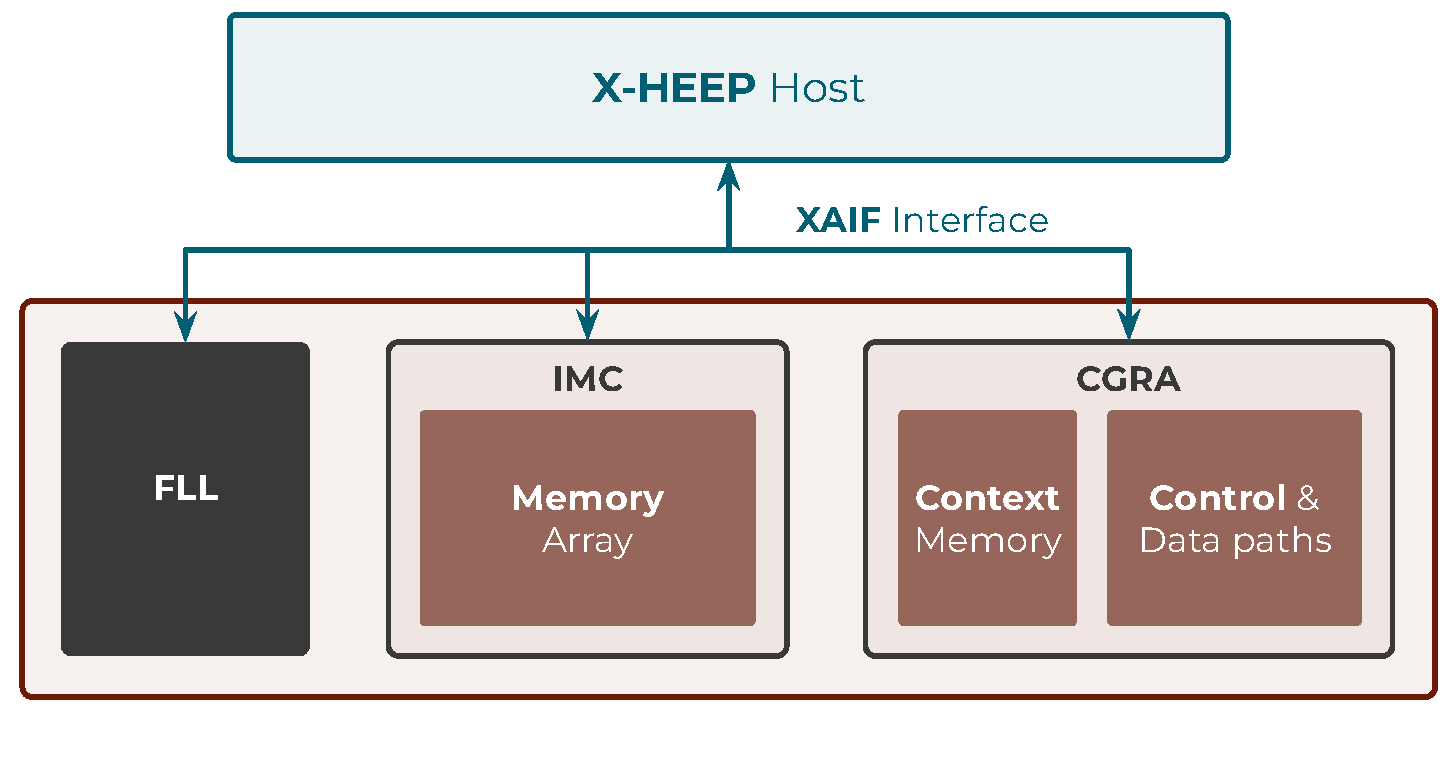
\includegraphics[width=0.8\textwidth]{./figures_x-heep/heepocrates.pdf}
                    \vspace{10px}
                    \caption{Block diagram of the \textit{HEEPocrates} architecture.}
                    \label{fig:heepocrates_block}
                \end{figure}

            \subsubsection*{CGRA accelerator}
            
                The CGRA~\cite{oe-cgra} integrated into \mbox{HEEPocrates} accelerates data-parallel signal processing tasks, such as filtering, convolutions, and matrix multiplications. It consists of a reconfigurable mesh of processing elements (PEs) and interfaces with the host through XAIF, providing a balance between programmability and energy efficiency suited to biomedical applications.
                
                The accelerator includes two OBI-compliant slave ports: one exposes control and status registers to the host, while the other is used to load PE instructions into a dedicated context memory. Each of the four PEs has an independent \SI{32}{\bit} OBI master port, allowing simultaneous access to the shared \mbox{X-HEEP} memory. This configuration achieves a total memory bandwidth of \SI{128}{\bit} per cycle, enabling efficient execution of low-latency streaming workloads.
                
                Synchronization between the CGRA and the host processor is handled via a dedicated XAIF interrupt. During kernel execution, the CPU can transition into a low-power sleep state and is automatically resumed upon task completion, thereby minimizing idle energy consumption.
                
                To further optimize energy proportionality, the CGRA architecture is divided into two power domains. The control and datapath domain supports both clock and power gating, allowing it to be completely powered down when idle. The context memory domain, by contrast, also supports retention, enabling context preservation across sparse execution phases without the need for reconfiguration. This separation enables efficient handling of intermittent workloads while keeping energy overheads low. Power state transitions are controlled via the XAIF interface, providing fine-grained runtime control in alignment with the bursty and event-driven nature of biomedical tasks.

            \vspace{-1em}
            \subsubsection*{IMC accelerator}
            
                The second accelerator integrated into \mbox{HEEPocrates} is an IMC engine~\cite{blade}, designed to enable ultra-low-power classification and inference by executing operations directly within memory arrays. This approach significantly reduces data movement and mitigates the energy inefficiencies associated with traditional Von Neumann architectures.
                
                The IMC connects to the system via a single OBI-compliant slave port, exposing its internal memory array to the host XAIF interface. This memory supports two distinct operating modes:

                \vspace{-1em}
                \begin{itemize}
                    \item \textbf{Memory Mode:} It operates as a standard read/write memory block, allowing the host or other compute units (e.g., the CGRA) to load data or retrieve computation results.
                    
                    \item \textbf{Computation Mode:} It activates embedded logic within the memory array to perform in-memory arithmetic operations directly on stored data, eliminating the need for data transfers and significantly lowering energy consumption.
                \end{itemize}
                \vspace{-1em}
                
                Mode transitions are managed autonomously by an embedded controller, abstracting low-level control details from the host and enabling streamlined software integration.
                
                The IMC is located in a dedicated power domain, with clock gating, power gating, and state retention capabilities exposed via the XAIF interface. This allows the accelerator to be powered down during idle acquisition phases and promptly reactivated for compute-intensive tasks, with optional context preservation.
                
                The combination of autonomous control, dual-mode memory functionality, and fine-grained power management makes the IMC accelerator particularly effective for biomedical tasks such as arrhythmia detection and sleep-stage classification, where energy efficiency and real-time responsiveness are critical.

                \vspace{-1em}
                \begin{figure}
                    \centering
                    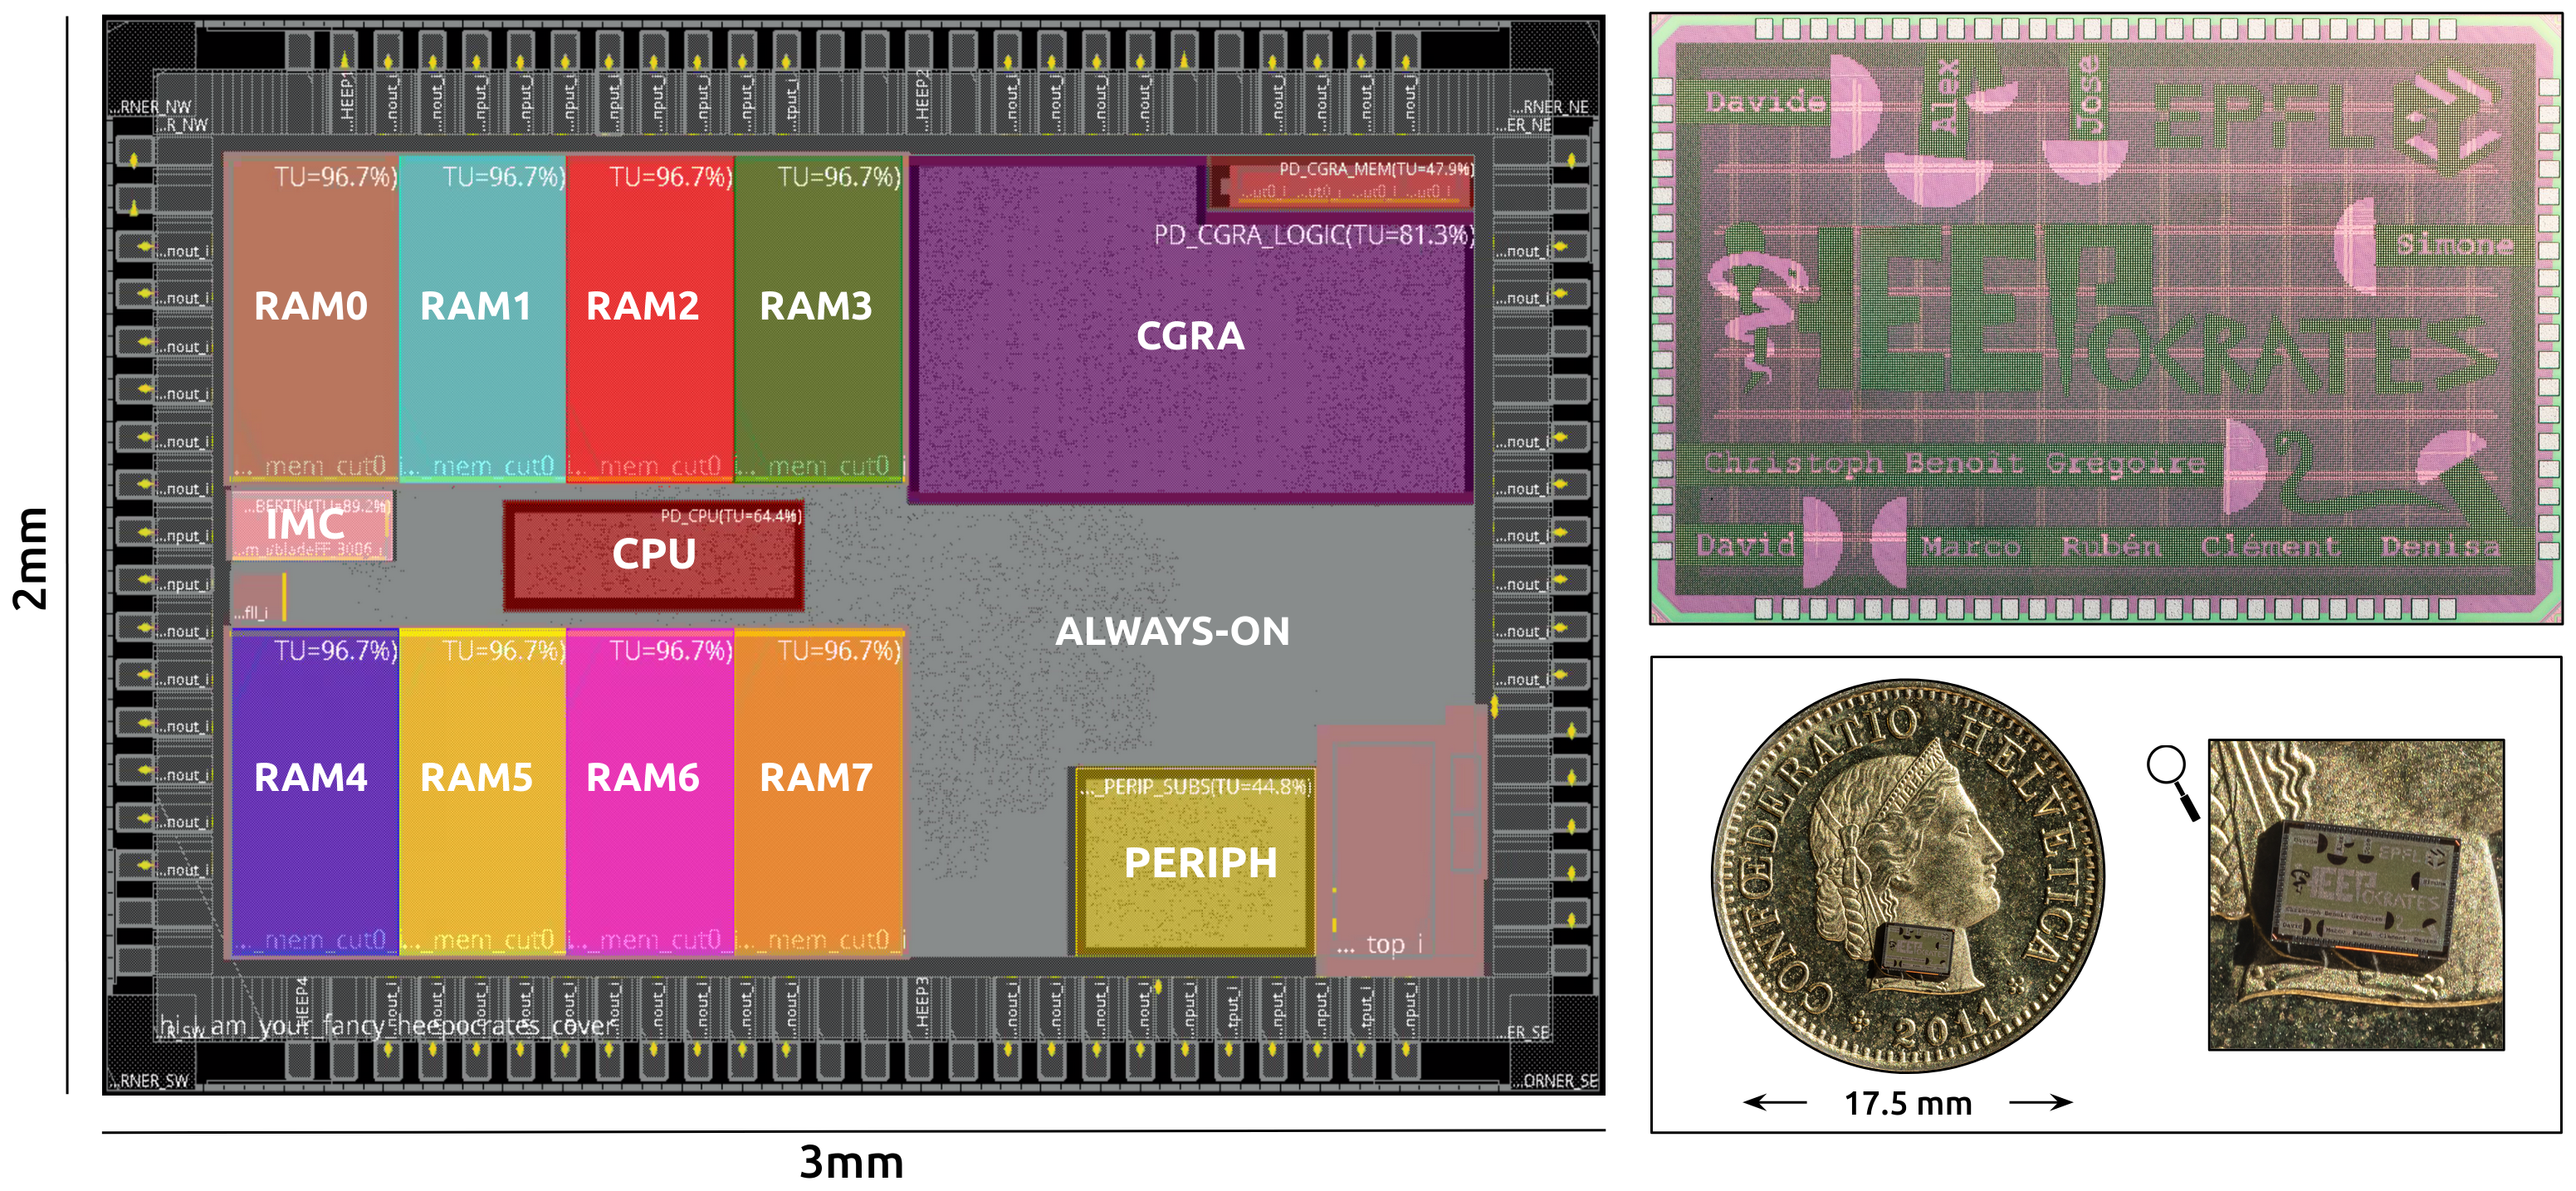
\includegraphics[width=1\textwidth]{./figures_x-heep/layout.png}
                    \vspace{5pt}
                    \caption{\textit{HEEPocrates} layout, silicon photo, and physical chip (on a Swiss 5-cent franc coin).}
                    \label{fig:layout}
                \end{figure}
                
            \subsubsection*{Frequency-locked loop}
            
                To enhance timing flexibility and energy efficiency, \mbox{HEEPocrates} integrates a programmable frequency-locked loop (FLL)~\cite{flleth} module, accessible through the XAIF interface. Implemented as a memory-mapped peripheral, the FLL enables dynamic control of the system clock frequency directly from the host.
                
                The module synthesizes a high-frequency system clock from a \SI{32}{\kilo\hertz} external crystal oscillator using a phase detector and control loop to ensure output stability. A software-accessible register interface supports real-time tuning of multiplication and division factors, enabling dynamic voltage and frequency scaling (DVFS)-like adjustments at the system level.
                
                This capability is particularly beneficial for biomedical applications. During low-demand acquisition phases, the system can operate at reduced frequency to minimize dynamic power, while higher clock rates can be enabled for compute-intensive tasks such as signal classification.
                
                Through fine-grained software control and seamless XAIF integration, the FLL delivers a low-overhead and efficient mechanism for system-wide energy scaling, a key requirement for battery-powered, energy-constrained healthcare platforms.

            \subsection{Implementation}
            
                \mbox{HEEPocrates} has been physically implemented and fabricated in the \mbox{TSMC} \SI{65}{\nano\meter} CMOS technology, resulting in a compact die area of \SI{6}{\milli\meter\squared} (\SI{3}{\milli\meter} $\times$ \SI{2}{\milli\meter}). Figure~\ref{fig:layout} illustrates the final implementation, including the layout view, the tapeout artwork, and a photograph of the packaged chip.
                
                The left portion of the layout hosts the eight SRAM banks (RAM0–RAM7), which are uniformly distributed to ensure balanced memory access and support power gating granularity. At the center of the die lies the \textsc{CV32E20} RISC-V CPU, which orchestrates system execution and accelerator control. In the bottom-left corner, the peripheral subsystem is located, interfacing with external sensors and communication buses.
                
                The top-right region integrates the CGRA, which is divided into logic and memory domains to support fine-grained power control. Just to the left of the CPU, the IMC accelerator is embedded, minimizing latency for memory-bound inference workloads.
                
                The top-right figure shows the final tapeout artwork, including project identifiers and designer signatures. Finally, the bottom-right image compares the size of the packaged chip to a Swiss 5-cent franc coin, highlighting its suitability for ultra-compact, battery-powered deployments.

    \section{Experimental Setup}
    \label{sec:experimental_setup}
    
        To validate the capabilities of the \mbox{X-HEEP} platform and its silicon instantiation as the \mbox{HEEPocrates} chip, a structured set of experiments is defined to characterize both design-time and run-time aspects of the system. These experiments span multiple abstraction levels, including RTL synthesis, physical implementation, and real-world application execution, offering a comprehensive evaluation of the platform.
        
        Specifically, the experimental setup is organized along three complementary axes that collectively assess configurability, physical behavior, and real-world applicability:

        \vspace{-1em}
        \begin{itemize}
            \item \textbf{X-HEEP characterization}: The \mbox{X-HEEP} platform is synthesized in a commercial \mbox{TSMC} \SI{65}{\nano\meter} CMOS technology. The analysis includes a detailed breakdown of area and leakage contributions from its internal components. In addition, multiple interconnect configurations are evaluated to assess the trade-offs between area and memory bandwidth. This exploration aims to:

            \begin{enumerate}[label=(\alph*)]
                \item Confirm the inherently low area and power overhead of the baseline \mbox{X-HEEP}, reinforcing its suitability as a host for TinyAI systems.
                \item Demonstrate the flexibility and scalability of the platform, enabling fine-grained optimization of performance, bandwidth, power, and area to meet diverse TinyAI application requirements.
            \end{enumerate}

            \item \textbf{HEEPocrates silicon characterization:} The physical behavior of the \mbox{HEEPocrates} SoC is evaluated by sweeping the operating voltage and frequency. This process extracts key parameters such as leakage current, switching power, and dynamic power density, providing a detailed energy profile of the chip.

            \item \textbf{HEEPocrates runtime characterization:} A suite of representative bio-signal processing applications, covering both idle and compute phases, is deployed on the fabricated \mbox{HEEPocrates} chip. These benchmarks, which include ECG and ECG feature extraction, reflect realistic edge healthcare workloads. Execution time and energy consumption are measured and compared with commercial ultra-low-power platforms to validate performance and efficiency.
        \end{itemize}
        \vspace{-1em}
        
        This three-pronged evaluation strategy provides a holistic assessment of the proposed platform. The design-space exploration highlights the configurability and design-time scalability of \mbox{X-HEEP}, while the silicon and run-time characterizations demonstrate the physical efficiency, functional completeness, and suitability for deployment in realistic edge TinyAI scenarios.

        \subsection{X-HEEP Characterization}

            This analysis quantifies the silicon footprint and leakage power of the \mbox{X-HEEP} platform and examines interconnect configurations to evaluate area–bandwidth trade-offs. All measurements are obtained through synthesis in a commercial \mbox{TSMC} \SI{65}{\nano\meter} CMOS technology using Synopsys Design Compiler, assuming a clock frequency of \SI{250}{\mega\hertz} and a supply voltage of \SI{1.2}{\volt}. The evaluation focuses on three complementary aspects:
            
            \vspace{-1em}
            \begin{itemize}
                \item \textbf{Area breakdown}: The total cell area is decomposed across the main architectural domains, CPU, memory, interconnect, peripheral blocks, and always-on modules. This breakdown identifies the most silicon-intensive components and highlights where selective instantiation or pruning can reduce the footprint without impacting essential functionality.
                
                \item \textbf{Leakage breakdown}: Leakage power is estimated under idle conditions for each major domain, including CPU, memory, interconnect, peripheral blocks, and always-on modules. The results quantify the static power contribution of each domain, providing a basis for applying domain-level power gating or other leakage mitigation strategies in duty-cycled or always-on workloads.
                
                \item \textbf{Interconnect exploration}: Two representative interconnect configurations are analyzed:~(i)~a one-at-a-time topology allowing one master–slave transaction at a time, and~(ii)~a fully connected topology supporting concurrent access from multiple masters to multiple memory ports. For each configuration, both total area and sustained memory bandwidth are measured under concurrent access patterns. This quantifies the trade-off between memory-level parallelism, critical for bandwidth-intensive workloads, and the associated hardware overhead.
            \end{itemize}
            \vspace{-1em}

        \subsection{HEEPocrates Silicon Characterization}
        
            To assess the physical behavior and energy efficiency of the \mbox{HEEPocrates} chip, a systematic post-silicon characterization is conducted. The campaign focuses on determining key operating parameters, including maximum functional frequency, minimum viable voltage, leakage power, and dynamic power density across a range of operating conditions.
            
            The \mbox{HEEPocrates} chip was fabricated using \mbox{TSMC} \SI{65}{\nano\meter} CMOS technology and mounted on a custom test board, shown in Figure~\ref{fig:test_board}. The board exposes standard interfaces for power and clock delivery, allowing integration with laboratory-grade instrumentation. A programmable power supply with sub-millivolt resolution and a variable-frequency clock generator provide precise operating conditions. Functional validation, test sequencing, and measurement control are orchestrated through firmware execution and GPIO-based signaling.

            \begin{figure} [t]
                \centering
                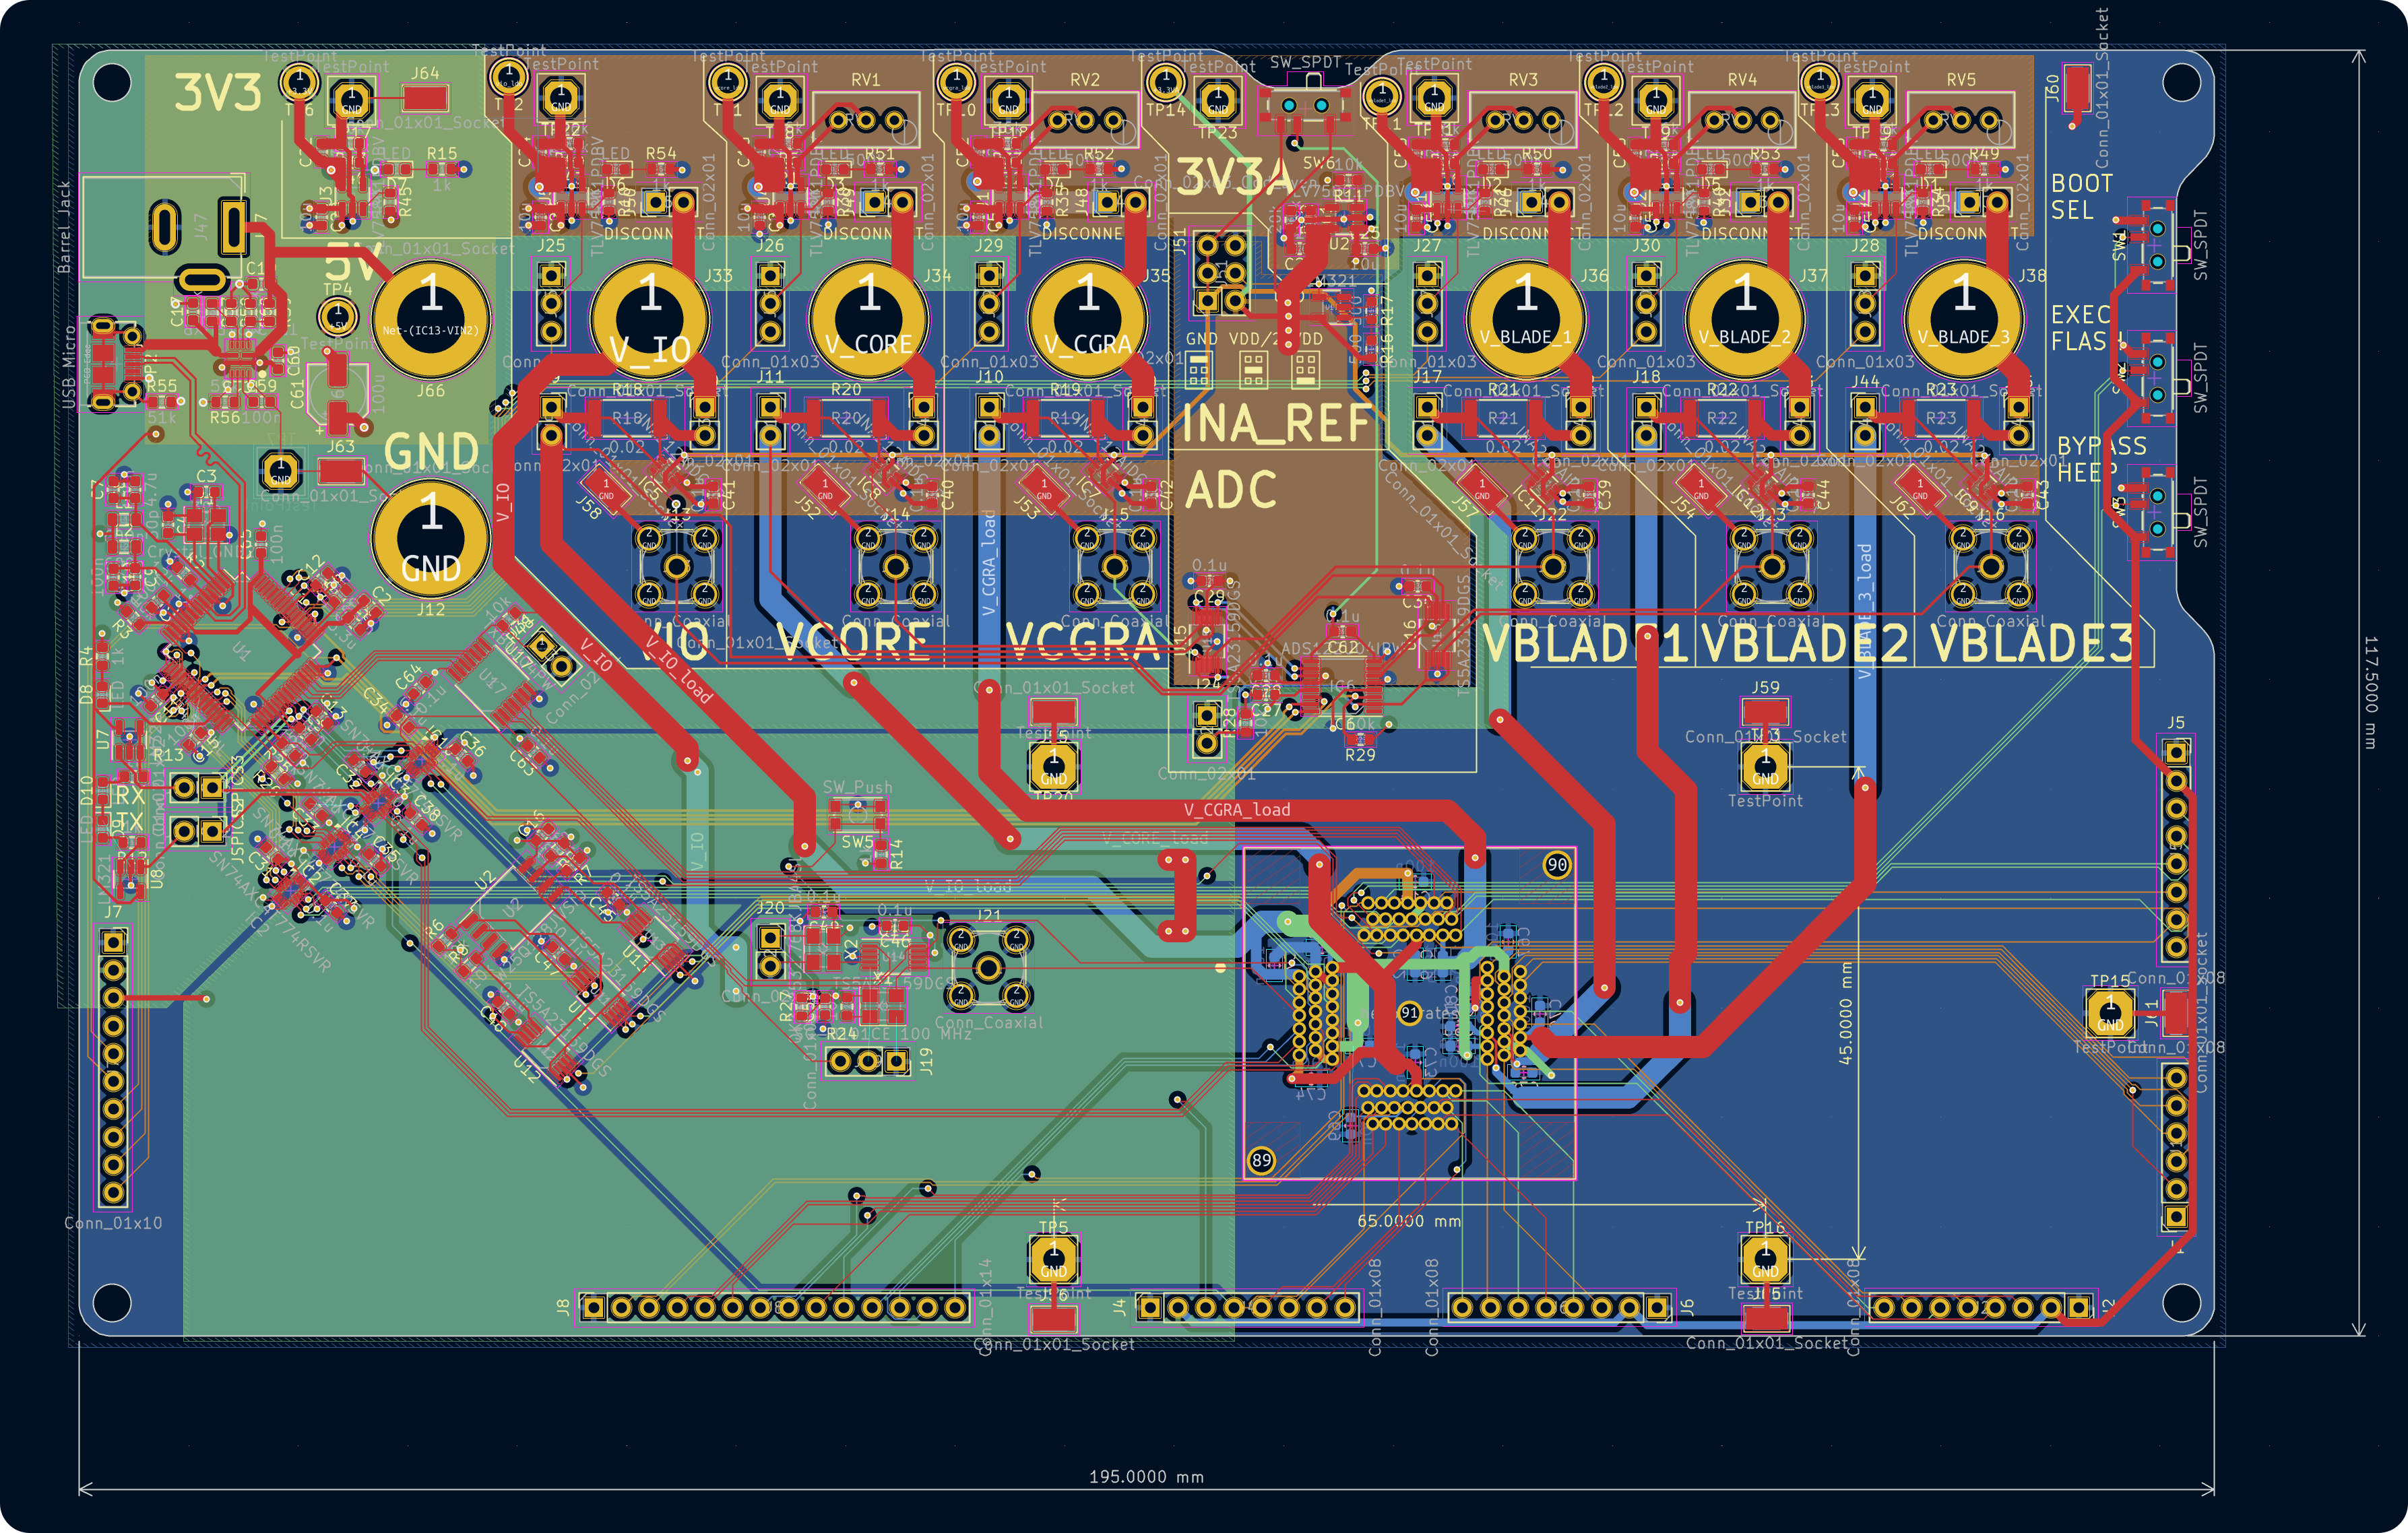
\includegraphics[width=0.8\textwidth]{./figures_x-heep/board.png}
                \caption{\textit{HEEPocrates} testing board under design.}
                \label{fig:test_board}
            \end{figure}
            
            The characterization procedure is organized into two main phases:

            \vspace{-1em}
            \begin{itemize}
                \item \textbf{Frequency and voltage range characterization:}
                
                The maximum stable operating frequency and the minimum functional supply voltage are determined using a representative matrix multiplication workload:
                
                \begin{enumerate}
                    \item Initialize the supply voltage at \SI{1.2}{\volt}.
                    
                    \item Load and execute the matrix multiplication kernel while incrementally increasing the input clock frequency.
                    
                    \item After each run, verify correctness using UART-based output comparison.
                    
                    \item If the kernel fails or stalls, record the last passing frequency as the maximum operating frequency for the given voltage.
                    
                    \item Repeat the process while gradually decreasing the supply voltage until the minimum voltage sustaining correct execution is identified.
                \end{enumerate}
            
                \item \textbf{Leakage and dynamic power density characterization:}
                
                Once the functional voltage-frequency range is identified, power measurements are conducted across all voltages from \SI{1.2}{\volt} down to the minimum operating point found in the previous step. At each voltage, current draw is measured at two distinct frequencies to extract dynamic and leakage components:
                
                \begin{enumerate}
                    \item Execute the kernel at the previously determined maximum frequency and measure the current to compute total power:
                    \[
                        P_{\text{max}} = V_{\text{DD}} \cdot I_{\text{max}}
                    \]
                    \item Repeat the measurement at a lower reference frequency (\SI{100}{\mega\hertz}) to determine the power:
                    \[
                        P_{100\text{MHz}} = V_{\text{DD}} \cdot I_{100\text{MHz}}
                    \]
                    \item Estimate dynamic power density \(D_y\) and leakage power \(P_{\text{lk}}\) by solving the linear power-frequency model:
                    \[
                        P = D_y \cdot f + P_{\text{lk}}
                    \]
                    \[
                        D_y = \frac{P_{\text{max}} - P_{100\text{MHz}}}{f_{\text{max}} - 100\text{MHz}}, \quad
                        P_{\text{lk}} = \frac{f_{\text{max}} \cdot P_{100\text{MHz}} - 100\text{MHz} \cdot P_{\text{max}}}{f_{\text{max}} - 100\text{MHz}}
                    \]
                \end{enumerate}
            
                All current measurements are acquired using precision instrumentation, and environmental conditions are kept constant throughout the experiments to ensure measurement accuracy.
            \end{itemize}

        \subsection{HEEPocrates Run-Time Characterization}
            
            The run-time characterization measures the performance and energy efficiency of the fabricated \mbox{HEEPocrates} chip under realistic operating conditions. This analysis targets complete application workloads, including both idle and processing phases, and compares the results with representative commercial ultra-low-power platforms to position \mbox{HEEPocrates} within the current state of the art~\cite{biomed}. All platforms are configured to their optimal operating points, and unused peripherals are disabled to minimize leakage.

            \vspace{-1em}
            \subsubsection*{Target platform}

                The testing board integrates the \mbox{HEEPocrates} chip, featuring a CV32E20 CPU~\cite{zeroriscy} together with on-chip CGRA~\cite{oe-cgra} and IMC~\cite{blade} accelerators. In this study, only the CPU is used, with all accelerators disabled. Application code and data are stored entirely in the on-chip \SI{256}{\kibi\byte} SRAM when possible, or partially in external SPI Flash otherwise. Peripheral domains and unused SRAM banks are power-gated during execution. The host CPU operates at \SI{470}{\mega\hertz} and \SI{1.2}{\volt} during processing phases, and its frequency is reduced to \SI{1}{\mega\hertz} during idle periods.
            
            \subsubsection*{Reference platforms}
            
                Five embedded platforms are selected to provide representative coverage of the host-based design space for ultra-low-power bio-signal processing. Their basic features and optimal core configurations are summarized in Table~\ref{tbl:platforms}, and a brief description of each platform is provided:

                \begin{table}[tp]
                    \caption{Summary of features and operating parameters of the selected platforms.}
                    \label{tbl:platforms}
                    \centering
                    \resizebox{\textwidth}{!}{
                    \begin{tabular}{|l|l|l|c|c|c|c|l|}
                    \toprule
                    \bf Board & \bf MCU & \bf Cores & \bf FPU & \shortstack{\bf RAM \\ \bf (KiB)} & \shortstack{\bf FLASH \\ \bf (MB)} & \shortstack{\bf Supply \\ \bf voltage (V)} & \shortstack{\bf Optimal core \\ \bf configuration} \\
                    \midrule
                    Ambiq             & Apollo 3 Blue    & 1x ARM Cortex-M4      & Yes & 384  & 1        & 1.8 (SoC)    & 0.7 V, 48 MHz   \\
                    Nucleo            & STML4R5ZI        & 1x ARM Cortex-M4      & Yes & 640  & 2        & 3.3 (SoC)    & 1.2 V, 120 MHz  \\
                    Gapuino           & GAP8             & 1x CV32E40P           & No  & 512  & off-chip & 2.8 (SoC)    & 0.8 V, 150 MHz  \\
                    GAP9EVK           & GAP9             & 1x CV32E40P           & Yes & 1564 & off-chip & 2.8 (SoC)    & 0.65 V, 240 MHz \\
                    Raspberry Pi Pico & RP2040           & 2x ARM Cortex-M0+     & No  & 264  & off-chip & 2.75 (Board) & 0.9 V, 133 MHz  \\
                    \midrule
                    HEEPocrates Dev   & HEEPocrates      & 1x CV32E20            & No  & 256  & off-chip & 1.2 (SoC)    & 0.8 V, 170 MHz \\
                    \bottomrule
                    \end{tabular}
                    }
                \end{table}

                \vspace{-1em}
                \begin{itemize}
                    \item \textbf{Ambiq}: The Apollo 3 Blue features a single ARM Cortex-M4 core with floating-point support, operating at \SI{48}{\mega\hertz} and \SI{0.7}{\volt} in the optimal configuration. It offers \SI{384}{\kibi\byte} of SRAM and \SI{1}{\mega\byte} of on-chip Flash. Its ultra-low-power design leverages aggressive clock and power gating, with an SoC nominal supply voltage of \SI{1.8}{\volt}.
                
                    \item \textbf{Nucleo}: Built around the STM32L4R5ZI SoC, it integrates a single ARM Cortex-M4 core with hardware floating-point support. The optimal configuration runs at \SI{120}{\mega\hertz} and \SI{1.2}{\volt}, providing \SI{640}{\kibi\byte} of SRAM and \SI{2}{\mega\byte} of on-chip Flash memory. The SoC operates at a nominal supply voltage of \SI{3.3}{\volt}.
                
                    \item \textbf{Gapuino}: Powered by the GAP8 SoC, this board combines a single CV32E40P~\cite{ri5cy} fabric controller core without floating-point support, clocked at \SI{150}{\mega\hertz} and \SI{0.8}{\volt}, with an 8-core CV32E40P compute cluster (unused in this study). The memory hierarchy includes \SI{512}{\kibi\byte} of shared L2 SRAM and \SI{64}{\kibi\byte} of private L1 SRAM. Program and data storage rely on off-chip Flash. The SoC operates at a nominal voltage of \SI{2.8}{\volt}.
                
                    \item \textbf{GAP9}: The GAP9EVK board is based on the GAP9 SoC, featuring a CV32E40P~\cite{ri5cy} fabric controller core with floating-point support, and a 9-core CV32E40P compute cluster (unused in this study). Both the fabric controller and cluster cores operate at \SI{240}{\mega\hertz} and \SI{0.65}{\volt} in the optimal configuration. The SoC integrates \SI{1564}{\kibi\byte} of shared L2 SRAM and \SI{128}{\kibi\byte} of private L1 SRAM per cluster core. Code and data are stored in off-chip Flash. The SoC nominal voltage is \SI{2.8}{\volt}.

                    \item \textbf{Raspberry Pi Pico}: Based on the RP2040 SoC, this platform integrates two ARM Cortex-M0+ cores without floating-point support, clocked at \SI{133}{\mega\hertz} at \SI{0.9}{\volt} in the optimal configuration. It features \SI{264}{\kibi\byte} of on-chip SRAM organized into multiple banks to enable concurrent access, while application code and data are stored in off-chip QSPI Flash. The board operates at a nominal supply voltage of \SI{2.75}{\volt}, with on-board regulation to the core domain.
                \end{itemize}
                \vspace{-1em}
                
                All experiments are executed exclusively on the CPU cores of the selected platforms, with any available hardware accelerators kept disabled. This choice ensures a fair comparison focused on the efficiency of the silicon implementation of the \mbox{X-HEEP} host within \mbox{HEEPocrates}, rather than comparing the accelerators present in the reference platforms.

            \subsubsection*{Benchmark suite}
            
                This evaluation employs the \emph{BiomedBench} benchmark suite~\cite{biomed}, a collection of representative biomedical applications that span various sensing modalities, computational kernels, and duty cycle requirements. The selected workloads include signal processing, feature extraction, and machine learning inference, covering a broad spectrum of computational intensities and memory footprints. Their main parameters are summarized in Table~\ref{tbl:x-heep_benchmarks}, and a brief description of each application is provided:

                \vspace{-1em}
                \begin{itemize}
                    \item \textbf{HeartBeatClass}: A real-time ECG classification workload implementing morphological filtering and complex detection, followed by heartbeat classification. It operates at a low duty cycle, sampling \SI{256}{\hertz} across three channels, and uses \SI{25}{\kibi\byte} of static memory with \SI{30}{\kibi\byte} of dynamic memory. Its main operations are time-domain filtering and pattern matching, making it representative of continuous cardiac monitoring systems.
                
                    \item \textbf{SeizDetSVM}: An EEG-based seizure detection pipeline featuring frequency-domain feature extraction using FFT, statistical computation, and classification via a support vector machine (SVM). Operating at a low duty cycle with a single channel at \SI{64}{\hertz}, it has modest memory requirements (\SI{40}{\kibi\byte} static and \SI{40}{\kibi\byte} dynamic). The design is optimized for long-term wearable operation under tight energy budgets.
                
                    \item \textbf{SeizDetCNN}: A CNN-based seizure detection application processing multi-channel EEG data. With a medium duty cycle, \SI{256}{\hertz} sampling rate, and 23 input channels, this workload imposes heavier demands on compute throughput and memory bandwidth. It requires \SI{300}{\kibi\byte} of static memory and \SI{120}{\kibi\byte} of dynamic memory, representing compute-bound edge AI inference tasks.
                
                    \item \textbf{CognWorkMon}: A cognitive workload monitoring pipeline that processes multi-channel EEG data through feature extraction and FFT to estimate mental workload levels in real time. It operates at a low duty cycle, sampling \SI{256}{\hertz} across four channels, with \SI{90}{\kibi\byte} static memory and \SI{50}{\kibi\byte} dynamic memory, balancing compute intensity with memory usage.
                
                    \item \textbf{GestureClass}: An inertial measurement unit (IMU)-based gesture classification workload performing multi-axis signal decomposition and classification. It features a high duty cycle, \SI{4000}{\hertz} sampling rate on 16 channels, and requires \SI{50}{\kibi\byte} static and \SI{110}{\kibi\byte} dynamic memory, stressing both real-time processing and memory access patterns.
                \end{itemize}
                \vspace{-1em}

                \begin{table}[tp]
                    \caption{Summary of characteristics of the applications in the benchmark.}
                    \label{tbl:x-heep_benchmarks}
                    \centering
                    \resizebox{\textwidth}{!}{
                    \begin{tabular}{|l|l|c|c|c|c|}
                    \toprule
                    \bf Application & \bf Main Tasks & \bf Duty Cycle &
                    \shortstack{\bf Sample rate \\ \bf (Hz) / \#Channels} &
                    \shortstack{\bf Static memory \\ \bf (KiB)} &
                    \shortstack{\bf Dynamic memory \\ \bf (KiB)} \\
                    \midrule
                    HeartBeatClass & Morphological filtering & Low      & 256 / 3   & 25  & 30  \\
                    SeizDetSVM     & Feat. extrac., FFT, SVM & Low      & 64 / 1    & 40  & 40  \\
                    SeizDetCNN     & CNN                     & Medium   & 256 / 23  & 300 & 120 \\
                    CognWorkMon    & Feature extraction, FFT & Low      & 256 / 4   & 90  & 50  \\
                    GestureClass   & Signal decomposition    & High     & 4000 / 16 & 50  & 110 \\
                    \bottomrule
                    \end{tabular}
                    }
                \end{table}
            
            \subsubsection*{Measurement methodology}
            
                Power consumption is recorded using high-precision current-sensing hardware integrated into each board or through an external digital power analyzer with sub-microsecond sampling resolution. Each workload is executed at least ten times to capture variability. All tests are conducted under stable ambient temperature and supply voltage conditions to avoid thermal drift and measurement artifacts.

    \section{Experimental Results}
    \label{sec:experimental_results}
        
        This section reports the results obtained from the experimental campaign described in Section~\ref{sec:experimental_setup}, covering the design-time configurability, silicon-level characterization, and run-time performance of the \mbox{X-HEEP} platform and its fabricated \mbox{HEEPocrates} implementation. The evaluation spans three complementary perspectives. First, the architectural flexibility of \mbox{X-HEEP} is examined through detailed analyses of area distribution, leakage breakdown, and interconnect topology, enabling a clear understanding of different design trade-offs. Second, the post-silicon characterization of \mbox{HEEPocrates} is presented, including voltage–frequency scaling behavior, total and leakage power measurements, and dynamic power density across representative workloads. Third, the run-time efficiency of \mbox{HEEPocrates} is benchmarked against widely used embedded platforms in the healthcare domain, with execution time and energy consumption broken down into processing and idle phases to capture the impact of workload duty cycle on performance and efficiency.

        \begin{table}[tp]
            \caption{Area and leakage distributions among the internal components of the \mbox{X-HEEP platform}.}
            \label{tbl:pie}
            \centering
            \resizebox{0.8\textwidth}{!}{
            \begin{tabular}{|l|c|c|c|c|}
            \toprule
            \bf{Component} & \bf{Area (\si{\milli\meter\squared})} & \bf{Area (\%)} & \bf{Leakage (\si{\micro\watt})} & \bf{Leakage (\%)} \\
            \midrule
            Bank 0          & 0.033  & 22 & 12.18 & 42 \\
            Bank 1          & 0.033  & 22 & 12.18 & 42 \\
            AO Periph.      & 0.0315 & 21 & 1.74  & 6  \\
            CPU             & 0.027  & 18 & 1.45  & 5  \\
            Peripherals     & 0.0165 & 11 & 1.16  & 4  \\
            Bus             & 0.006  & 4  & 0.29  & 1  \\
            Debug           & 0.003  & 2  & 0.29  & 1  \\
            \midrule
            \bf{Total}      & \bf{0.15} & \bf{100} & \bf{29.29} & \bf{100} \\
            \bottomrule
            \end{tabular}
            }
        \end{table}

        \subsection{X-HEEP Characterization}
        
            The configurability and implementation efficiency of the \mbox{X-HEEP} platform are evaluated across three representative architectural dimensions: \emph{area distribution}, \emph{leakage distribution}, and \emph{interconnect topology}. Together, these analyses quantify the physical cost, static power profile, and communication scalability of the architecture, providing concrete guidance for design trade-offs in different TinyAI deployment scenarios.

            \vspace{-1em}
            \subsubsection*{Area breakdown}
        
                Table~\ref{tbl:pie} and Figure~\ref{fig:pie} show the area distribution among the internal components of the \mbox{X-HEEP} architecture, which occupies a total silicon area of \SI{0.15}{\milli\meter\squared}. The two memory banks dominate the design, accounting for a combined \SI{44}{\percent} of the area, with each bank contributing \SI{22}{\percent}. The always-on (AO) peripheral domain follows at \SI{21}{\percent}, providing essential system control and wake-up functionality, while the standard peripheral subsystem accounts for \SI{11}{\percent}. The CV32E20 CPU~\cite{zeroriscy} itself requires only \SI{18}{\percent} of the total area, and the bus and debug modules contribute minimal overhead of \SI{4}{\percent} and \SI{2}{\percent}, respectively.
        
                This breakdown confirms that the integration overhead of \mbox{X-HEEP} is low, with almost half the footprint dedicated to memory structures rather than control or computation logic. This profile is advantageous for embedded deployments, as memory size can be directly scaled to match the requirements of the target workload, enabling aggressive footprint reduction in memory-light applications.

                \begin{figure}[t]
                    \centering
                    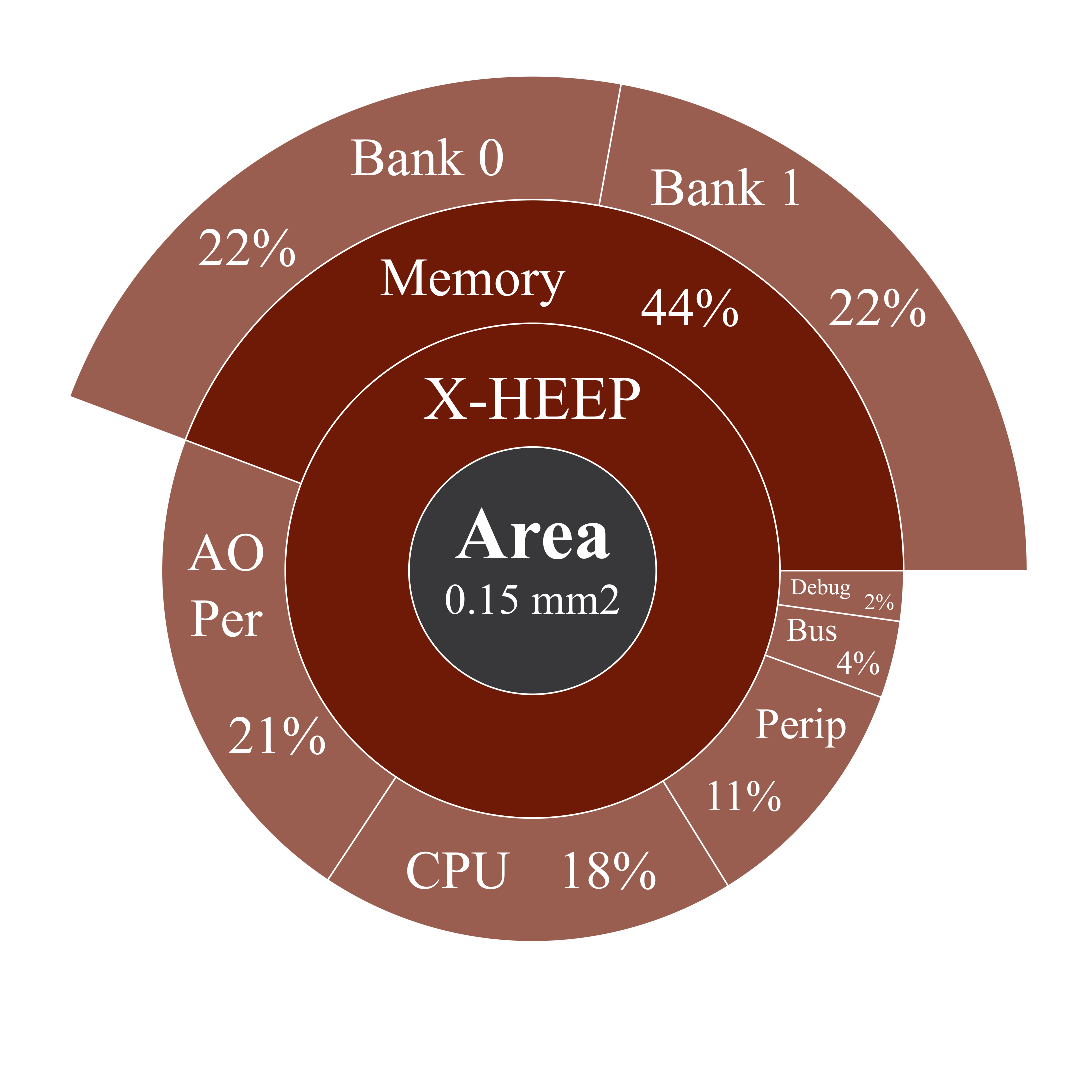
\includegraphics[width=0.4\textwidth]{./figures_x-heep/pie_area.pdf}
                    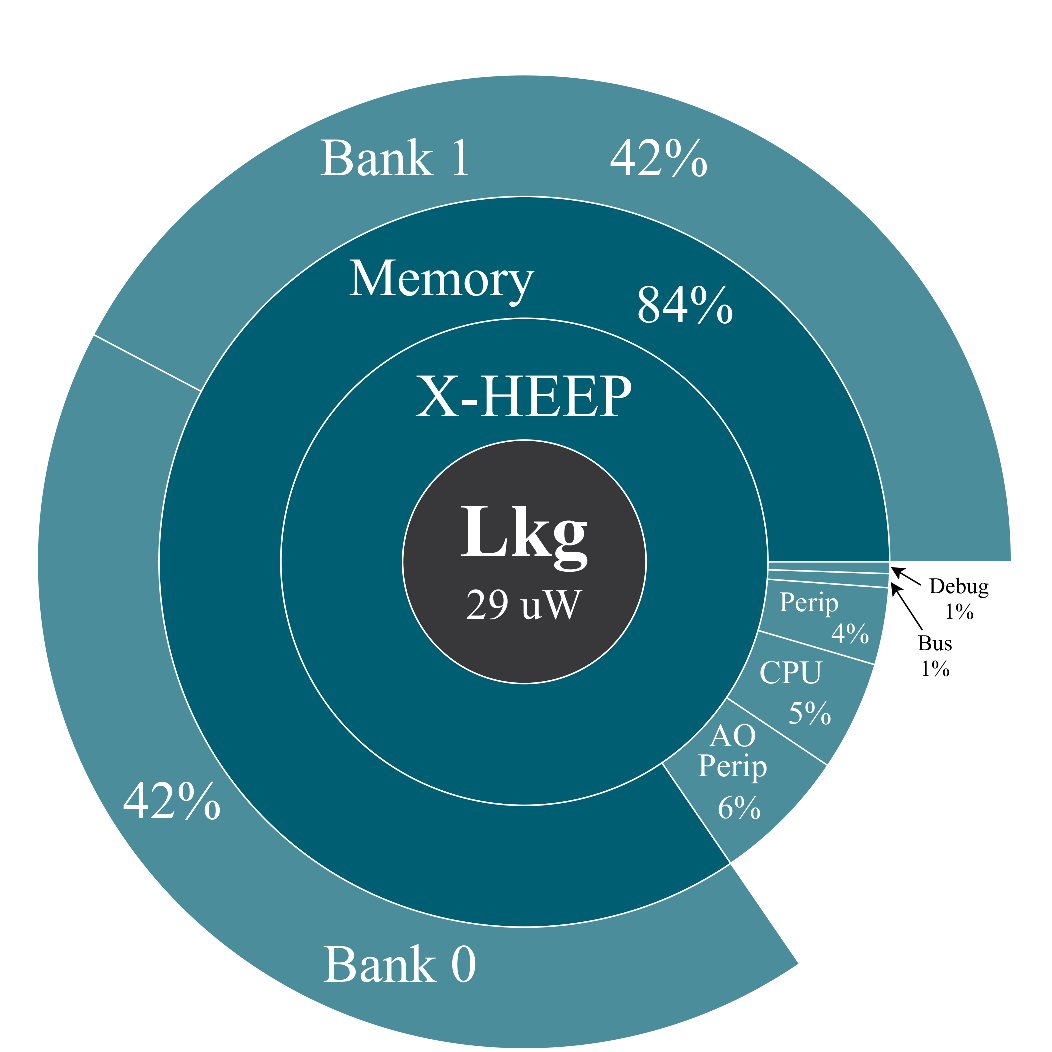
\includegraphics[width=0.4\textwidth]{./figures_x-heep/pie_leakage.pdf}
                    \caption{Area and leakage distributions among the internal components of the \mbox{X-HEEP platform}.}
                    \label{fig:pie}
                \end{figure}

            \vspace{-1em}
            \subsubsection*{Leakage breakdown}
        
                The leakage power profile of \mbox{X-HEEP} follows a similar pattern, with a total leakage of \SI{29}{\micro\watt}. The two memory banks are again the dominant contributors, responsible for a combined \SI{84}{\percent} of the leakage budget, evenly divided between them. The always-on peripheral domain accounts for \SI{6}{\percent}, ensuring continuous availability for wake-up and monitoring tasks, while the standard peripheral subsystem contributes \SI{4}{\percent}. The CPU core exhibits low static power consumption at \SI{5}{\percent}, and the bus and debug modules each contribute a negligible \SI{2}{\percent}.
        
                This distribution highlights the inherently low leakage overhead of the logic components, with static power concentrated mainly in the memory subsystem. Importantly, the CPU, peripherals, and individual memory banks can be independently power-gated through the power manager when not in use. In scenarios with aggressive duty cycling, this reduces total leakage to as little as \SI{3}{\micro\watt}, extending operational lifetime in battery-powered TinyAI devices.

            \vspace{-1em}
            \subsubsection*{Interconnect exploration}
            
                The scalability of the internal communication fabric is assessed by comparing two representative interconnect configurations: \emph{(i) a one-at-a-time bus}, and  
                \emph{(ii) a fully connected crossbar}. Table~\ref{tbl:bus} and Figures~\ref{fig:bus} summarize the results in terms of area and sustained memory bandwidth.
        
                The baseline configuration comprises the CV32E20~\cite{zeroriscy} core, two memory banks, a debug unit, and two peripheral domains. The number of master–slave port pairs is then increased incrementally (1M1S, 2M2S, …, 6M6S) to emulate increasingly heterogeneous system scenarios. Each additional master port is paired with an internal slave port, typically connected to a memory bank, to avoid contention on the memory side.

                \begin{table}[tp]
                    \caption{Comparison of area (kGE) and sustained memory bandwidth (bits/cycle) for different interconnect configurations.}
                    \label{tbl:bus}
                    \centering
                    \resizebox{0.8\textwidth}{!}{
                    \begin{tabular}{|c|c|c|c|c|}
                    \toprule
                    \multirow{2}{*}{\bf{Configuration}} & \multicolumn{2}{c|}{\bf{One-at-a-time}} & \multicolumn{2}{c|}{\bf{Fully connected}} \\
                    \cline{2-5}
                     & \bf{Area (kGE)} & \bf{BW (bits/cycle)} & \bf{Area (kGE)} & \bf{BW (bits/cycle)} \\
                    \midrule
                    1M1S & 1.1  & 32  & 7.8  & 32  \\
                    2M2S & 1.3  & 32  & 10.1 & 64  \\
                    3M3S & 1.4  & 32  & 12.5 & 96  \\
                    4M4S & 1.6  & 32  & 16.3 & 128 \\
                    5M5S & 1.8  & 32  & 19.5 & 160 \\
                    6M6S & 2.0  & 32  & 23.1 & 192 \\
                    \bottomrule
                    \end{tabular}
                    }
                \end{table}
        
                In the one-at-a-time configuration (Figure~\ref{fig:bus}(a)), the area grows modestly from \SI{1.1}{\kilogateequiv} in the 1M1S setup to \SI{2.0}{\kilogateequiv} in the 6M6S setup. This minimal increase reflects the simplicity of the arbitration logic and serialized communication. However, bandwidth remains fixed at \SI{32}{\bit/\cycle}, independent of the number of ports, revealing the fundamental concurrency limitation of this approach. While extremely area-efficient, it cannot support parallel transactions, limiting its applicability to low-throughput or latency-tolerant workloads.
        
                The fully connected configuration (Figure~\ref{fig:bus}(b)), by contrast, provides dedicated routing paths between each master–slave pair, enabling independent and concurrent data transfers. This yields a linear increase in sustained bandwidth, from \SI{32}{\bit/\cycle} in the 1M1S case to \SI{192}{\bit/\cycle} in the 6M6S case. The trade-off is a steep area cost, rising from \SI{7.8}{\kilogateequiv} to \SI{23.1}{\kilogateequiv}, driven by the quadratic growth in arbitration and multiplexing resources.
        
                Overall, this comparison exposes a clear trade-off between area efficiency and communication parallelism. The one-at-a-time topology is well-suited to ultra-low-power deployments with limited concurrency, whereas the fully connected topology targets compute-intensive scenarios with high memory bandwidth requirements. The modular design of \mbox{X-HEEP} allows the implementation or even the combination of the modules, based on the performance and efficiency goals of the target workload.

                \begin{figure} [t]
                    \centering
                    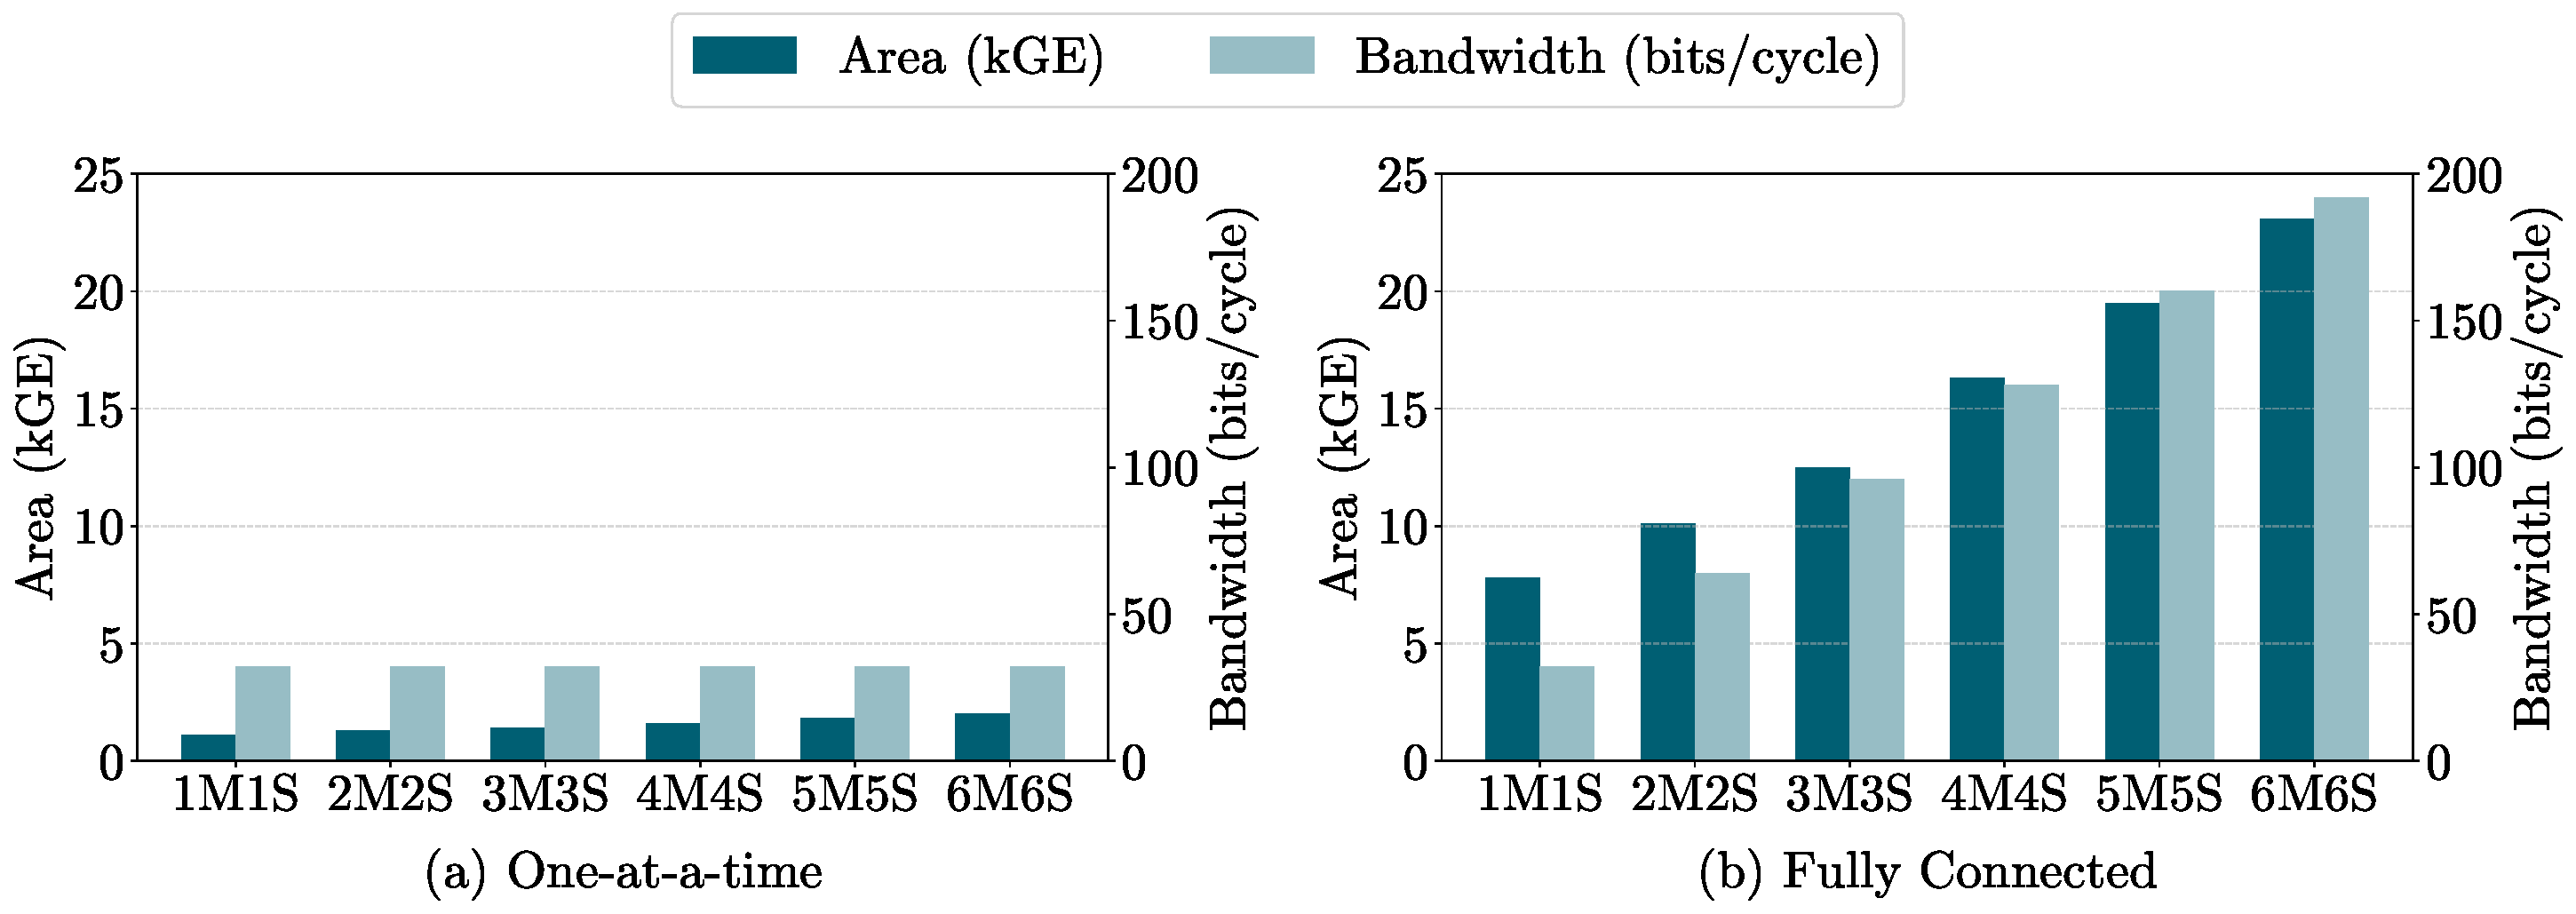
\includegraphics[width=1\textwidth]{figures_x-heep/bus.pdf}
                    \caption{Comparison of area (kGE) and sustained memory bandwidth (bits/cycle) for different interconnect configurations.}
                    \label{fig:bus}
                \end{figure}

        \subsection{HEEPocrates Silicon Characterization}
        
            Table~\ref{tbl:voltage_scaling} and Figure~\ref{fig:voltage_scaling} highlight key trends that define the operating envelope of the \mbox{HEEPocrates} chip. The maximum achievable frequency scales quasi-linearly with supply voltage, rising from approximately \SI{170}{\mega\hertz} at \SI{0.80}{\volt} to \SI{470}{\mega\hertz} at \SI{1.20}{\volt}. This behavior reflects the reduction in logic delay associated with higher overdrive voltages in standard-cell CMOS technology. The absence of saturation or discontinuities across the tested range confirms robust timing closure and the lack of critical path violations, thereby enabling a well-defined DVFS range in which software can reliably select the highest feasible frequency for any given voltage without violating timing constraints.
            
            Under full-load conditions, measured during the execution of a matrix multiplication kernel at maximum frequency, total power consumption increases superlinearly with voltage. It ranges from under \SI{8}{\milli\watt} at \SI{0.80}{\volt} to about \SI{48}{\milli\watt} at \SI{1.20}{\volt}. This steep increase results from the quadratic dependence of dynamic power on voltage, compounded by the higher switching activity at elevated frequencies. While performance scales linearly with voltage, the associated power cost escalates more rapidly, reducing energy efficiency at the upper end of the DVFS range. Identifying optimal operating points within this trade-off space is particularly relevant for energy-constrained edge workloads.
            
            The leakage power, measured in idle mode in the same voltage range, grows exponentially from \SI{366.86}{\micro\watt} at \SI{0.80}{\volt} to \SI{968.08}{\micro\watt} at \SI{1.20}{\volt}, consistent with the voltage sensitivity of the subthreshold and gate leakage in CMOS technologies. Although leakage remains a minor contributor during active computation, it dominates during idle or sleep phases, underscoring the importance of voltage scaling in always-on or low-duty-cycle applications.

            The dynamic power density, expressed in~\si{\micro\watt\per\mega\hertz}, was measured for four representative workloads: \emph{matrix multiplication (2MM)}, \emph{idle (NOP)}, \emph{wait-for-interrupt (WFI)}, and \emph{power-gated (PWG)}. This normalized metric isolates switching activity by expressing energy cost per unit frequency. All workloads exhibit a consistent upward trend, starting from \SI{43.37}{\micro\watt\per\mega\hertz} at \SI{0.80}{\volt} and reaching \SI{110.20}{\micro\watt\per\mega\hertz} at \SI{1.20}{\volt} for the most active kernel. The variation across applications reflects their computational intensity: 2MM and NOP, which maintain active processing states, exhibit substantially higher dynamic energy consumption than WFI or PWG, which spend most of their time in low-power sleep states.

            These measurements provide valuable insights for system-level modeling and DVFS policy design. The impact of operating at higher voltages varies significantly with workload characteristics: for lightweight tasks, the small performance gains are outweighed by increased power consumption, leading to reduced energy efficiency. In contrast, compute-bound workloads can benefit from short high-frequency bursts, completing execution faster and lowering overall energy consumption when the power budget allows.

            \begin{table}[tp]
                \caption{Voltage scaling impact on frequency, total power, leakage power, and dynamic power density for the \mbox{HEEPocrates} chip.}
                \label{tbl:voltage_scaling}
                \centering
                \resizebox{\textwidth}{!}{
                \begin{tabular}{|c|c|c|c|
                                >{\centering\arraybackslash}p{1.5cm}|
                                >{\centering\arraybackslash}p{1.5cm}|
                                >{\centering\arraybackslash}p{1.5cm}|
                                >{\centering\arraybackslash}p{1.5cm}|}
                \toprule
                \multirow{2}{*}{\bf Voltage (V)} & 
                \multirow{2}{*}{\bf Max. Freq. (MHz)} & 
                \multirow{2}{*}{\bf Total Power (mW)} & 
                \multirow{2}{*}{\bf Lkg Power ($\mu$W)} & 
                \multicolumn{4}{c|}{\bf Dynamic Power Density ($\mu$W/MHz)} \\
                \cline{5-8}
                 & & & & \bf 2MM & \bf NOP & \bf WFI & \bf PWG \\
                \midrule
                0.80 & 170 & 7.74  & 366.86 & 43.37 & 40.15 & 23.33 & 17.10 \\
                0.85 & 210 & 10.60 & 357.08 & 48.97 & 45.27 & 26.30 & 19.28 \\
                0.90 & 250 & 14.10 & 370.20 & 55.00 & 50.63 & 29.53 & 21.66 \\
                0.95 & 290 & 18.20 & 406.45 & 61.40 & 56.46 & 33.01 & 24.17 \\
                1.00 & 330 & 23.00 & 463.30 & 68.39 & 62.72 & 36.59 & 26.81 \\
                1.05 & 360 & 27.80 & 567.81 & 75.64 & 69.36 & 40.55 & 29.69 \\
                1.10 & 400 & 34.00 & 692.27 & 83.21 & 76.30 & 44.60 & 32.68 \\
                1.15 & 440 & 41.00 & 819.88 & 91.22 & 83.59 & 48.85 & 35.82 \\
                1.20 & 470 & 48.10 & 968.08 & 100.20 & 91.50 & 53.52 & 39.26 \\
                \bottomrule
                \end{tabular}
                }
            \end{table}

            \begin{figure}[t]
                \centering
                \begin{subfigure}{1\textwidth}
                    \centering
                    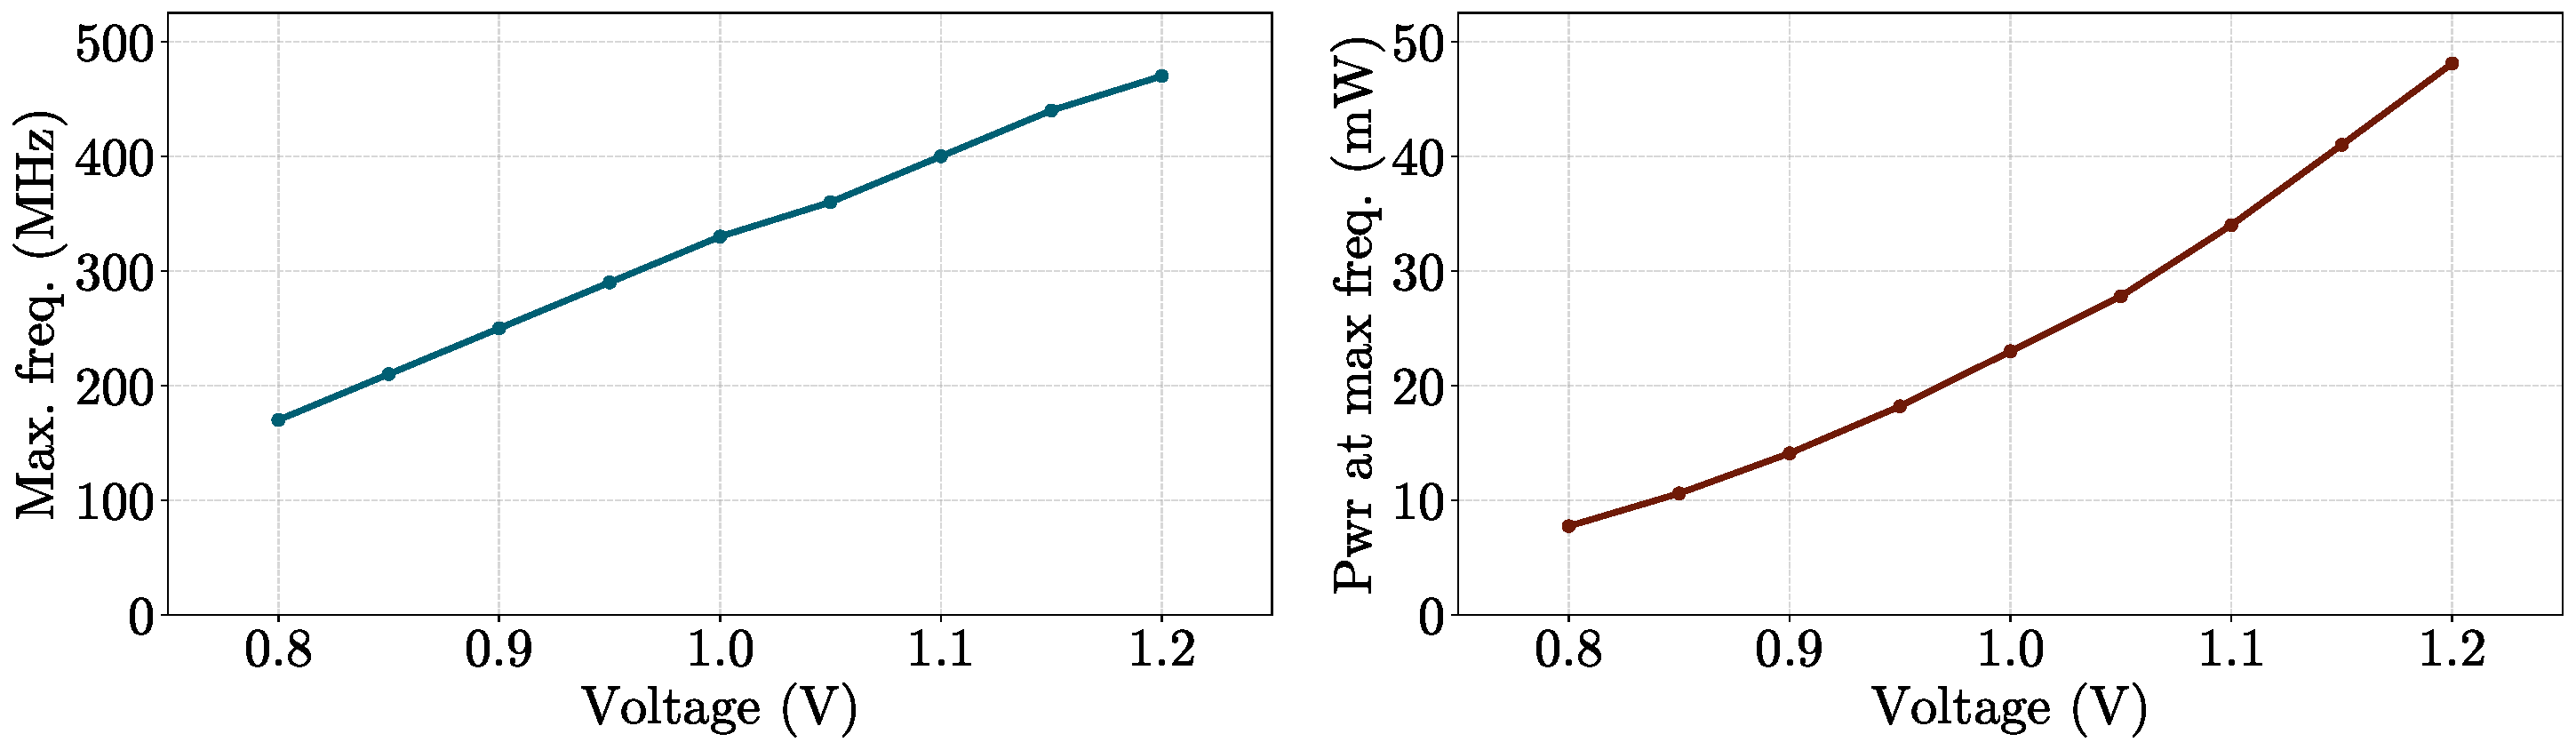
\includegraphics[width=1\textwidth]{./figures_x-heep/freq_pwr.pdf}
                    \label{fig:freq_pwr}
                \end{subfigure}
                \vspace{1em}
                \begin{subfigure}{\textwidth}
                    \centering
                    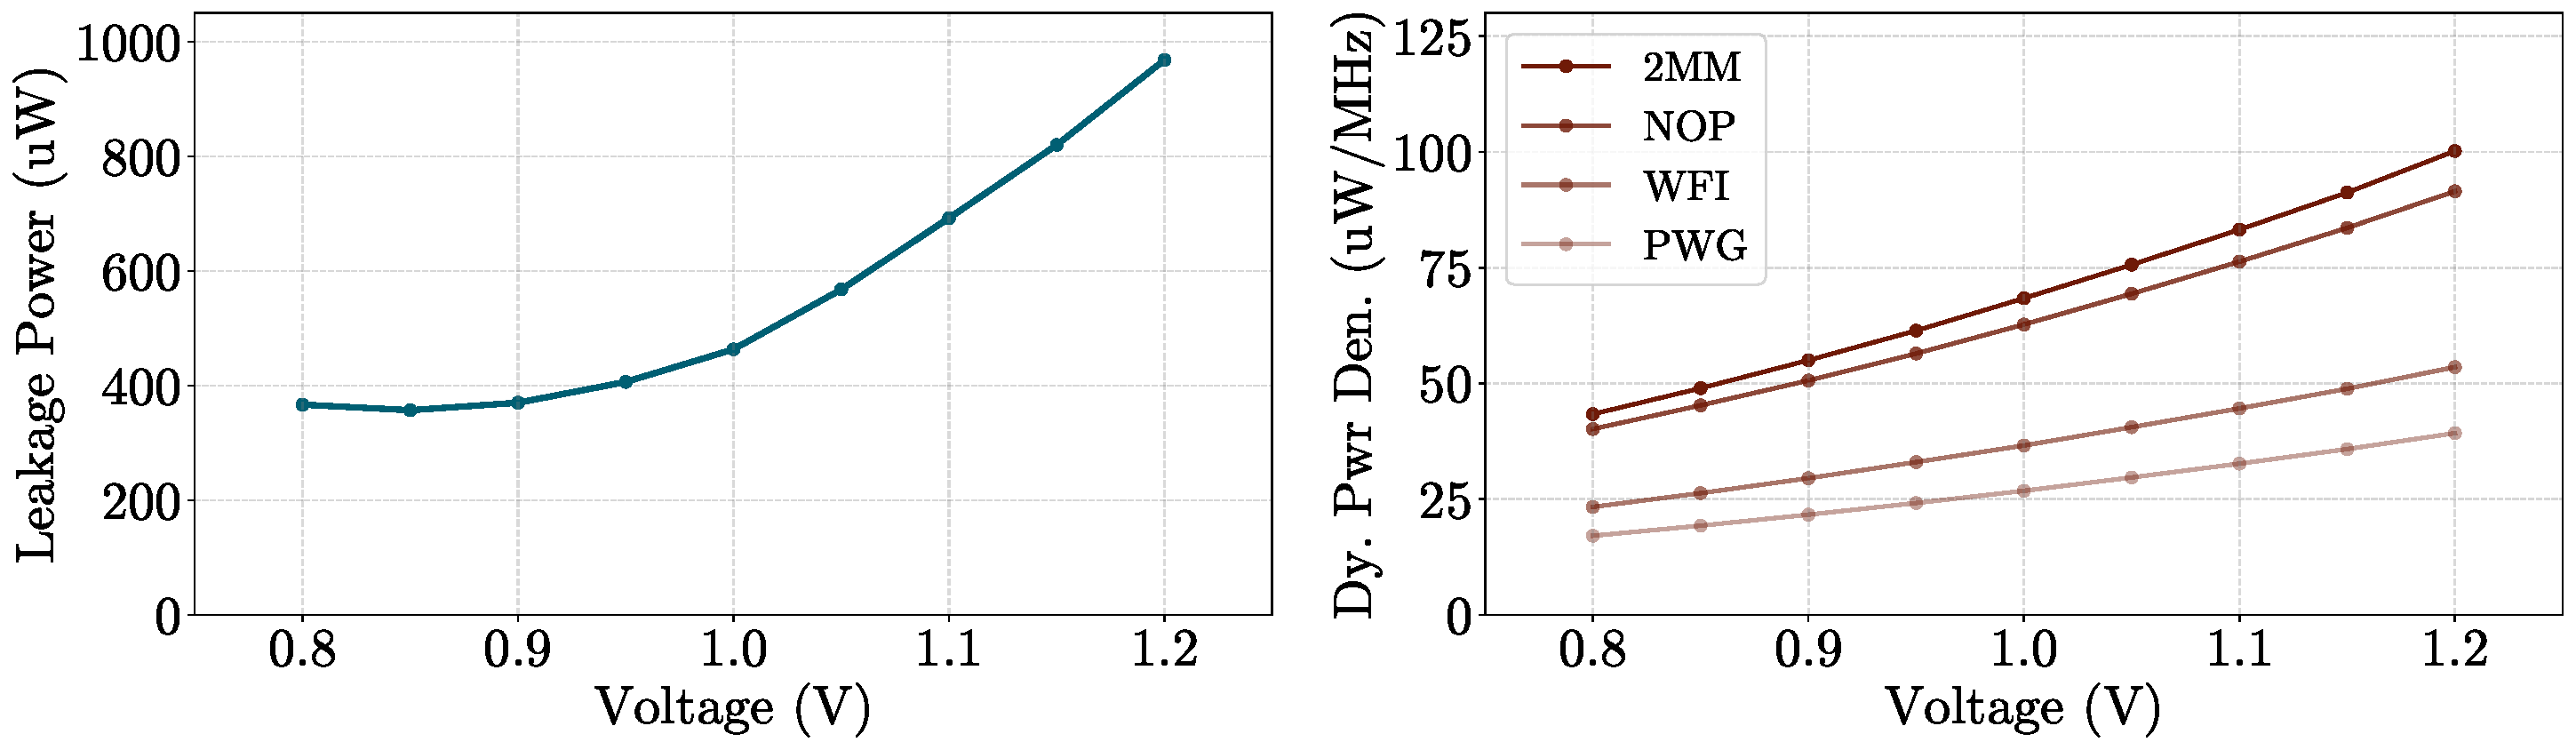
\includegraphics[width=1\textwidth]{./figures_x-heep/lkg_dyn.pdf}
                    \label{fig:lkg_dyn}
                \end{subfigure}
                \caption{Voltage scaling impact on frequency, total power, leakage power, and dynamic power density for the \mbox{HEEPocrates} chip.}
                \label{fig:voltage_scaling}
            \end{figure}
            
        \subsection{HEEPocrates Run-Time Characterization}
        
            In the evaluated workloads, execution is structured into two non-overlapping active phases: the \emph{processing} phase, during which the system executes the computational pipeline on the current input window, and the \emph{idle} phase, in which the system remains in a low-power state while waiting for the next window to be ready for processing. Data acquisition is performed concurrently with both phases using a double-buffering strategy: while one buffer is being processed, the next buffer is being filled with new sensor data. As a result, the acquisition phase is fully overlapped with the processing and idle periods, and its energy cost is implicitly included in the energy figures of these two phases. All benchmarks are executed on the CPU of each platform, without leveraging any multi-core processing or hardware accelerators.

            Figure~\ref{fig:proc_energy} and Tables~\ref{tbl:time}--\ref{tbl:energy} summarize the measured execution times and energy consumption, split into processing (P) and idle (I) contributions, for all benchmarks and platforms. In low-duty-cycle workloads such as HeartBeatClass, SeizDetSVM, and CognWorkMon, idle time accounts for more than \SI{94}{\percent} of total execution time. For example, in HeartBeatClass, \mbox{HEEPocrates} spends \SI{14.981}{\second} idle and \SI{0.019}{\second} processing, compared to Apollo3 \SI{14.885}{\second} idle and \SI{0.115}{\second} processing. While \mbox{HEEPocrates} achieves a shorter processing time due to a higher operating frequency, Apollo3 consumes far less total energy (\SI{0.36}{\milli\joule} versus \SI{11.71}{\milli\joule}) thanks to its aggressive clock-gating and power-gating strategies. A similar trend appears in SeizDetSVM, where \mbox{HEEPocrates} processes in \SI{0.009}{\second} for \SI{0.435}{\milli\joule}, but idle energy dominates at \SI{43.253}{\milli\joule} because its leakage is higher than in Apollo3. In CognWorkMon, \mbox{HEEPocrates} completes processing in \SI{0.338}{\second}, outperforming STM32L4 \SI{1.172}{\second} due to its higher frequency, but idle energy still represents the majority of consumption (\SI{40.132}{\milli\joule}).
            
            In the medium-duty-cycle \texttt{SeizDetCNN}, processing accounts for a significant fraction of the total execution time. In this case, \mbox{HEEPocrates} completes processing in \SI{0.879}{\second} and idles for \SI{3.121}{\second}, consuming \SI{42.290}{\milli\joule} in processing and only \SI{2.250}{\milli\joule} in idle. The reduced processing time compared to STM32L4 (\SI{2.010}{\second}) and RP2040 (\SI{1.451}{\second}) can be attributed to its higher sustained memory bandwidth. As a result, total energy consumption (\SI{44.54}{\milli\joule}) is significantly lower than STM32L4 (\SI{112.07}{\milli\joule}) and RP2040 (\SI{178.91}{\milli\joule}), with further gains enabled by its aggressive frequency scaling.

            \begin{table}[tp]
                \caption{Execution time (s) for each benchmark, split into processing (Proc) and idle (Idle) phases across all platforms. Negative idle times indicate that the processing duration exceeds the task deadlines.}
                \label{tbl:time}
                \centering
                \resizebox{\textwidth}{!}{
                \begin{tabular}{|c|
                                c|c|
                                c|c|
                                c|c|
                                c|c|
                                c|c|
                                c|c|}
                \toprule
                \multirow{2}{*}{\bf Application} & 
                \multicolumn{2}{c|}{\bf Apollo} & 
                \multicolumn{2}{c|}{\bf STM} & 
                \multicolumn{2}{c|}{\bf GAP8} & 
                \multicolumn{2}{c|}{\bf GAP9} & 
                \multicolumn{2}{c|}{\bf RP} & 
                \multicolumn{2}{c|}{\bf HEEPocrates} \\
                \cline{2-13}
                 & {\bf Proc} & {\bf Idle} & {\bf Proc} & {\bf Idle} & {\bf Proc} & {\bf Idle} & {\bf Proc} & {\bf Idle} & {\bf Proc} & {\bf Idle} & {\bf Proc} & {\bf Idle} \\
                \midrule
                HeartBeatClass & 0.115 & 14.885 & 0.046 & 14.954 & 0.026 & 14.974 & 0.012 & 14.988 & 0.045 & 14.955 & 0.019 & 14.981 \\
                SeizDetSVM     & 0.059 & 59.941 & 0.023 & 59.977 & 0.009 & 59.991 & 0.003 & 59.997 & 0.022 & 59.978 & 0.009 & 59.991 \\
                SeizDetCNN     & 2.341 & 1.659  & 2.010 & 1.990  & 0.232 & 3.768  & 0.070 & 3.930  & 1.451 & 2.549  & 0.879 & 3.121 \\
                CognWorkMon    & 2.930 & 53.070 & 1.172 & 54.828 & 1.617 & 54.383 & 0.608 & 55.392 & 2.600 & 53.400 & 0.338 & 55.662 \\
                GestureClass   & 0.239 & \textcolor{myred}{-0.039}  & 0.191 & 0.009  & 1.015 & \textcolor{myred}{-0.815}  & 0.011 & 0.189  & 2.529 & \textcolor{myred}{-2.329}  & 2.198 & \textcolor{myred}{-1.998} \\
                \bottomrule
                \end{tabular}
                }
            \end{table}

            \begin{table}[tp]
                \caption{Energy consumption (mJ) for each benchmark, split into processing (Proc) and idle (Idle) phases across all platforms. Zero idle times indicate that the processing duration exceeds the task deadlines.}
                \label{tbl:energy}
                \centering
                \resizebox{\textwidth}{!}{
                \begin{tabular}{|c|
                                c|c|
                                c|c|
                                c|c|
                                c|c|
                                c|c|
                                c|c|}
                \toprule
                \multirow{2}{*}{\bf Application} & 
                \multicolumn{2}{c|}{\bf Apollo} & 
                \multicolumn{2}{c|}{\bf STM} & 
                \multicolumn{2}{c|}{\bf GAP8} & 
                \multicolumn{2}{c|}{\bf GAP9} & 
                \multicolumn{2}{c|}{\bf RP} & 
                \multicolumn{2}{c|}{\bf HEEPocrates} \\
                \cline{2-13}
                 & {\bf Proc.} & {\bf Idle} & {\bf Proc.} & {\bf Idle} & {\bf Proc.} & {\bf Idle} & {\bf Proc.} & {\bf Idle} & {\bf Proc.} & {\bf Idle} & {\bf Proc.} & {\bf Idle} \\
                \midrule
                HeartBeatClass & 0.230 & 0.130 & 0.230 & 0.120 & 0.822 & 9.431  & 0.411 & 9.987  & 0.411 & 33.166 & 0.911 & 10.801 \\
                SeizDetSVM     & 0.137 & 0.336 & 1.313 & 0.477 & 0.353 & 37.772 & 0.179 & 39.604 & 2.420 & 121.207 & 0.435 & 43.253 \\
                SeizDetCNN     & 18.262 & 0.504 & 112.049 & 0.019 & 31.987 & 0.554 & 5.101 & 2.351 & 167.870 & 11.042 & 42.290 & 2.250 \\
                CognWorkMon    & 3.887 & 0.945 & 70.629 & 0.449 & 16.008 & 34.361 & 3.711 & 36.860 & 195.910 & 140.778 & 16.275 & 40.132 \\
                GestureClass   & 2.500 & \textcolor{myred}{0.000} & 13.425 & 0.004 & 220.933 & \textcolor{myred}{0.000} & 0.604 & 0.151 & 347.104 & \textcolor{myred}{0.000} & 105.709 & \textcolor{myred}{0.000} \\
                \bottomrule
                \end{tabular}
                }
            \end{table}
            
            In the high-duty-cycle GestureClass, processing time frequently exceeds the acquisition window, resulting in missed real-time deadlines. This behavior appears in Table~\ref{tbl:time} as negative idle times (highlighted in red), indicating that processing for a given window completes only after the next acquisition window has already started. For example, \mbox{HEEPocrates} requires \SI{2.198}{\second} for processing and reports \SI{-1.998}{\second} idle, consuming \SI{105.709}{\milli\joule} during processing. While \mbox{HEEPocrates} cannot match the throughput of GAP9 in this workload (\SI{0.011}{\second} processing), it achieves lower energy consumption than GAP8 (\SI{220.93}{\milli\joule}) and RP2040 (\SI{347.10}{\milli\joule}).
            
            Overall, the results confirm that different platforms excel in different workload profiles: ultra-low-leakage systems such as Apollo3 dominate in idle-heavy, low-duty-cycle applications due to their minimal static power; general-purpose systems like STM32L4 and RP2040 achieve higher throughput for compute-intensive tasks but pay an energy penalty from higher dynamic and leakage power; and \mbox{HEEPocrates} offers a balanced alternative. Although it cannot match the idle efficiency of the most aggressively power-gated platforms, it delivers competitive or superior processing performance in medium- to high-duty-cycle scenarios, demonstrating alignment with established state-of-the-art platforms commonly adopted in the bio-signal processing domain.

            \begin{figure}[t]
                
\includegraphics[width=1\textwidth]{./figures_x-heep/proc_energy.pdf}
                \caption{Energy consumption of our benchmark running on common healthcare microcontrollers and on \mbox{HEEPocrates} at \SI{0.8}{\volt}. P: Processing; I: Idle.}
                \label{fig:proc_energy}
            \end{figure}

    \section{X-HEEP-based Systems}
    \label{sec:x-heep_based_systems}
    
        The versatility of the \mbox{X-HEEP} platform has made it a reference host architecture for a wide variety of heterogeneous computing solutions. Its modular design, parameterizable interconnect, and flexible memory hierarchy provide a robust yet adaptable foundation for integrating accelerators, supporting hardware–software co-design, and validating emerging computing paradigms for TinyAI workloads. Over the past few years, \mbox{X-HEEP} has been used both as a rapid prototyping environment for FPGA-based evaluations and as the basis for multiple silicon implementations.
        
        This section is organized into two complementary parts. The \emph{Accelerator Exploration} subsection surveys representative research works that exploit the platform to investigate diverse accelerator integration strategies. The \emph{Chip Gallery} subsection provides an overview of fabricated \mbox{X-HEEP}-based tapeouts, showcasing the range of technology nodes and application domains achieved with the platform.

        \subsection{Accelerator Exploration}
        
            The works presented here showcase how \mbox{X-HEEP} has been employed as a host platform to integrate domain-specific accelerators targeting a wide range of domains, including machine learning, signal processing, arithmetic, and biomedical computing. These examples, while not exhaustive, illustrate how the \mbox{X-HEEP} highly configurable architecture, modular memory hierarchy, and well-defined integration interfaces enable efficient prototyping and in-depth exploration of state-of-the-art accelerator concepts for TinyAI systems. To highlight different design philosophies, the selected works are grouped into three categories based on their coupling strategy with the host: \emph{slave-only accelerators}, which operate solely under CPU control and process data received from the host; \emph{master/slave hybrid accelerators}, which can both autonomously initiate memory transactions and respond to host commands; and \emph{tightly coupled coprocessors}, which integrate directly into the CPU pipeline through ISA extensions or dedicated interfaces.
            
            \subsubsection*{Slave-only Accelerators}
                
                Slave-only accelerators are controlled entirely by the host CPU, receiving data and commands through memory-mapped registers or DMA transfers, and returning results for further processing. This approach benefits from the \mbox{X-HEEP} modular memory subsystem, which allows SRAM banks to be transparently replaced by compute-capable modules without requiring modifications to the bus protocol or software infrastructure.
                
                The near-memory computing (NMC)~\cite{nmc} work illustrates this integration style by embedding two accelerators, NM-Caesar and NM-Carus, directly in place of standard \SI{32}{\kibi\byte} SRAM banks, preserving interface, timing, and pinout to minimize integration complexity. NM-Caesar is a compact, SIMD-enabled unit controlled by the host CPU or DMA for low-complexity workloads, whereas NM-Carus integrates a small RISC-V core and vector unit to execute preloaded kernels via a custom NMC-oriented ISA autonomously. In \mbox{X-HEEP}, both accelerators connect transparently to the system bus, with NM-Carus supporting interrupt-driven execution for asynchronous operation. Post-layout results in \SI{65}{\nano\meter} show NM-Caesar achieving up to \SI{28}{\times} speedup and \SI{25}{\times} energy gains, and NM-Carus up to \SI{54}{\times} speedup and \SI{36}{\times} energy gains over the CPU baseline, demonstrating the benefits of seamless NMC integration in TinyML workloads.
                
                While NMC brings compute to SRAM banks, the HEEPstor framework~\cite{systolic_array} demonstrates how \mbox{X-HEEP} can host a slave-only accelerator specialized for a specific computation pattern: general matrix multiplication (GEMM) in quantized machine learning workloads. HEEPstor integrates a hybrid-quantized systolic array tightly coupled to the CV32E40P RISC-V core~\cite{ri5cy} via a memory-mapped interface. Dedicated bridge modules connect the OBI system bus to the accelerator command interface, ensuring a clean separation from the rest of the SoC. On the software side, HEEPstor automates the deployment of unmodified PyTorch models by applying \SI{8}{\bit} post-training quantization to weights, converting layers into GEMM-friendly operations, and generating optimized C++ inference code targeting the \mbox{X-HEEP}+accelerator platform. FPGA-based evaluations on Fashion-MNIST show that a $16 \times 16$ systolic array configuration achieves up to \SI{4.5}{\times} speedup for large CNN models while preserving baseline accuracy after quantization, confirming the suitability of \mbox{X-HEEP} for rapid hardware–software co-design.
            
            \subsubsection*{Master/Slave Hybrid Accelerators}
            
                Master/slave hybrid accelerators expand beyond the slave-only model by incorporating the ability to initiate memory transactions autonomously, often through DMA, while still accepting explicit commands from the host CPU. This configuration allows for more autonomous data movement and reduced CPU intervention, improving throughput and energy efficiency. The \mbox{X-HEEP} modular interconnect and the DMA controller provide the flexibility needed for such designs.
                
                The STRELA project~\cite{strela} exemplifies this category by integrating a lightweight RISC-V–based SIMD accelerator aimed at ultra-low power parallel execution of regular data-parallel kernels. Its architecture features a simple control core coupled to a \SI{16}{}-lane SIMD unit, optimized for minimal area and leakage. In \mbox{X-HEEP}, STRELA is instantiated as a memory-mapped peripheral on the system interconnect, using DMA-driven data transfers from shared SRAM banks to feed the SIMD pipelines. This structure allows direct CPU control through custom registers without altering the host memory subsystem. Fabricated in \SI{65}{\nano\meter}, STRELA adds less than \SI{0.04}{\milli\meter\squared} of area and \SI{6}{\micro\watt} of leakage, while achieving up to \SI{12}{\times} speedup and \SI{11}{\times} energy savings over the CPU baseline for representative vectorizable workloads.
                
                Taking hybrid autonomy further, the TestIt framework~\cite{dma} integrates a smart peripheral controller (SPC) with tight coupling to the DMA engine to accelerate the \textit{im2col} transformation for convolutional layers. By exploiting the DMA 2D transfer capability, the SPC can sequentially fetch and reshape feature map data into matrix form, enabling convolutions to be executed as single GEMM operations. Within \mbox{X-HEEP}, the SPC is connected as a custom peripheral on the system bus, with direct DMA interfacing to the shared SRAM banks for high-throughput data movement. The TestIt framework validates this integration through a combination of simulation and FPGA prototyping, reducing the test campaign time by \SI{11}{\times} compared to RTL simulation and exposing subtle hardware/software interaction issues, such as protocol synchronization faults in DMA HAL functions, that would otherwise go undetected.
                
                Expanding the hybrid model to always-on vision processing, the Percival accelerator~\cite{percival} targets sub-\SI{}{\milli\watt} convolutional neural network inference for wearable and IoT devices. Fabricated in \SI{16}{\nano\meter}, Percival implements a binary-weight CNN datapath optimized for minimal bandwidth and storage requirements while maintaining accuracy. Integrated into \mbox{X-HEEP} as a memory-mapped peripheral, it connects to the system interconnect and shared SRAM banks, with the CV32E40P host core~\cite{ri5cy} managing configuration, scheduling, and DMA-based data streaming. This arrangement enables real-time vision inference with up to \SI{30}{\times} energy efficiency gains over the CPU baseline.
                
                Complementing this vision-oriented design, the Athos accelerator~\cite{athos} addresses reconfigurable biomedical signal processing, specifically ECG-based arrhythmia detection. Like Percival, it connects to \mbox{X-HEEP} as a memory-mapped peripheral, but leverages DMA-driven transfers from shared SRAM banks to feed its configurable processing pipeline. Athos supports multiple operating modes, from full-precision to compressed feature extraction, allowing accuracy–energy trade-offs. Its autonomous operation is facilitated by \mbox{X-HEEP} clock-domain management and flexible peripheral interface. Implemented in \SI{65}{\nano\meter}, Athos achieves up to \SI{22}{\times} speedup and \SI{15}{\times} energy savings over the CPU baseline, highlighting the versatility of \mbox{X-HEEP} in hosting dynamically reconfigurable biomedical accelerators.
            
            \subsubsection*{Tightly Coupled Coprocessors}
            
                Tightly coupled coprocessors integrate directly into the CPU pipeline, enabling low-latency offloading of specialized operations via ISA extensions or dedicated execution hooks. In \mbox{X-HEEP}, such designs are supported by the XIF coprocessor interface, which allows custom functional units to share the CPU register file and instruction stream.
                
                The ARCANE accelerator~\cite{arcane} extends the near-memory computing paradigm into the cache hierarchy by replacing the standard LLC with multiple NM-Carus–based vector processing units (VPUs) managed by an embedded RISC-V controller. These VPUs execute kernels using a software-defined matrix ISA, with the host CPU offloading complex in-cache instructions through the XIF interface. ARCANE autonomously manages data movement, synchronization, and cache coherence, enabling concurrent execution of host and in-cache tasks without explicit application-level memory handling. Implemented in \SI{65}{\nano\meter}, ARCANE incurs a \SIrange{21}{41}{\percent} area overhead depending on VPU count, and achieves up to \SI{84}{\times} speedup over a scalar CPU and \SI{16}{\times} over a SIMD/DSP-enhanced core for large \SI{8}{\bit} convolutional layers, with sustained performance gains on large datasets due to reduced data movement.
                
                Quadrilatero~\cite{quadrilatero} represents a matrix-oriented coprocessor designed to address the bandwidth and register-file access limitations of vector processors in matrix-heavy workloads. Quadrilatero connects to \mbox{X-HEEP} via the XIF interface, working alongside the CV32E40PX core~\cite{ri5cy} and multi-banked SRAM subsystem. Offloaded matrix instructions are executed on a $4 \times 4$ systolic array with dedicated load/store and permutation units, enabling high-throughput data movement between the matrix register file and shared memory. In \SI{65}{\nano\meter}, Quadrilatero occupies only \SI{0.65}{\milli\meter\squared}, reaches up to \SI{99.4}{\percent} FPU utilization, delivers \SI{3.87}{\times} speedup, and achieves up to \SI{77}{\percent} area efficiency gains and \SI{15}{\percent} energy savings compared to contemporary vector or hybrid vector–matrix designs.

        \subsection{Chip Gallery}
            
            Beyond FPGA-based prototyping, the \mbox{X-HEEP} platform has served as the foundation for a diverse set of fabricated systems-on-chip, each tailored to different research goals, technology nodes, and accelerator architectures. These tapeouts demonstrate the adaptability of the platform to a wide range of integration styles, from analog front ends to coarse-grained reconfigurable arrays and safety-critical processing islands. While the author of this thesis has been directly involved in the design and development of \mbox{HEEPocrates} and \mbox{HEEPatia}, other \mbox{X-HEEP}-based silicon implementations produced by collaborating research groups are also presented, each embedding custom accelerators to target specific application domains. A detailed overview of these tapeouts, including their architectural configurations, integrated accelerators, and implementation technologies, is provided in Appendix~\ref{appendix:chip_gallery}.

    \section{Summary and Conclusions}
    \label{sec:conclusions}
    
        This chapter has presented \mbox{X-HEEP}, an open-source, highly configurable, and extendible platform designed to facilitate the integration and exploration of TinyAI accelerators. The design addresses two key limitations of existing open-source host platforms: the lack of fine-grained architectural configurability and the absence of standardized, scalable interfaces for accelerator integration. By adopting a modular architecture and a parameterized RTL structure, \mbox{X-HEEP} enables application-specific tailoring of CPU type, memory organization, interconnect topology, peripheral sets, and power domains, without the need for manual RTL modification.  
        
        A central contribution is the introduction of the XAIF interface, a standardized integration layer supporting a wide range of accelerator types, from loosely coupled memory-mapped units to tightly coupled ISA extensions. XAIF consolidates communication, synchronization, and low-power control mechanisms into a unified interface abstraction, significantly reducing integration effort and verification complexity. This approach enables the integration of compute units with varying performance, memory, and energy needs, while maintaining modularity and reusability.
        
        The applicability of the platform has been demonstrated through \mbox{HEEPocrates}, a representative bio-signal processing SoC integrating a CGRA~\cite{oe-cgra} and an IMC~\cite{blade} accelerator. Implemented in TSMC \SI{65}{\nano\meter} CMOS technology, \mbox{HEEPocrates} showcases the suitability of the platform for real-world, ultra-low-power deployments. The integration leverages XAIF to provide uniform connectivity, dedicated power domains, and fine-grained clock/power gating, ensuring that energy consumption scales proportionally with workload demands, an essential requirement for duty-cycle biomedical applications.
        
        The experimental campaign validated the platform from three complementary perspectives:
        
        \vspace{-1em}
        \begin{itemize}
            \item \textbf{X-HEEP characterization:} Designed to serve as a flexible host for TinyAI heterogeneous systems, \mbox{X-HEEP} was evaluated to quantify its integration cost, leakage profile, and scalability. The baseline configuration occupies only \SI{0.15}{\milli\meter\squared} and dissipates \SI{29}{\micro\watt} of leakage power, while its modular memory system and configurable interconnect enable fine-grained area–bandwidth trade-offs. This allows the architecture to be tailored to the performance and efficiency needs of diverse workloads.
        
            \item \textbf{HEEPocrates silicon characterization:} To support energy-aware workload scheduling, the fabricated \mbox{HEEPocrates} SoC was characterized for functional operating range and power–performance scaling. It maintains stable operation from \SI{0.8}{\volt} to \SI{1.2}{\volt}, with maximum frequencies of \SI{170}{\mega\hertz} and \SI{470}{\mega\hertz}, respectively. Total power increases from \SI{7.8}{\milli\watt} at \SI{170}{\mega\hertz} and \SI{0.8}{\volt} to \SI{48}{\milli\watt} at \SI{470}{\mega\hertz} and \SI{1.2}{\volt}, providing a broad DVFS envelope for optimizing performance and energy efficiency.
        
            \item \textbf{HEEPocrates run-time evaluation:} The platform was benchmarked on representative TinyAI bio-signal processing workloads to assess real-world performance and energy efficiency against state-of-the-art ultra-low-power systems. \mbox{HEEPocrates} delivers competitive or superior processing efficiency in medium- and high-duty-cycle applications, while its idle leakage remains higher than that of the most aggressively power-gated SoC. These results confirm its suitability for compute-intensive edge healthcare workloads requiring both high throughput and flexible execution modes.
        \end{itemize}
        \vspace{-1em}
        
        In summary, \mbox{X-HEEP} advances the state-of-the-art in open-source host platforms for TinyAI by combining high architectural configurability, a standardized and extendible accelerator interface, and ASIC-ready implementation flows. Its release as a publicly available, fully documented framework fosters reproducibility and accelerates research on heterogeneous systems at the edge. The silicon-proven \mbox{HEEPocrates} implementation demonstrates that these design principles are effectively translated into competitive, energy-efficient platforms suitable for deployment in real-world applications. This combination of configurability, extensibility, and implementation readiness establishes \mbox{X-HEEP} as a versatile foundation for exploring domain-specific accelerators and next-generation TinyAI systems.
